\section{Numerical implementation} \label{sec:numerical_implementation}

As discussed in \sec{sec:radial_locality}, the radial kernels decay ($\propto ~ \beta^{-1.5}$) as the distance from the central pixel increases, but they begin to increase on approaching the diametrically opposite position ($\beta \rightarrow \pi$)  as seen in \fig{fig:rad_ker_decay}. For a map containing sufficiently high multipole $\ell_{\rm max}$ information,  the local maxima the radial kernel attains in the vicinity of the diametrically opposite end is significantly smaller than global maxima. This suggests that for sufficiently high resolution CMB maps, it may suffice to restrict the convolution over the Stoke parameters Q \& U to a local region around the central pixel. The size of this local region is determined by the non-locality parameter $\beta_o$. \revisit{It is important to note that this claim is valid only while working with maps that are fairly homogeneous. In the case of foregrounds for example, though the radial kernel falls off, a strong foreground very far from the central pixel may still make significant contribution to the local definition of E and B modes.}

In this section we study the effects of localizing the convolution kernels on the inferred E and B mode maps and their power spectra. We have developed a Python script to compute these local convolution over Stokes Q \& U parameters. To carry out this numerical exercise, we pre-compute the radial part of the kernels, namely the function: $f(\beta), {}_{+2}f(\beta) ~\&~ {}_{-2}f(\beta)$. We use the python routine {\textit scipy.special.lpmn} for the numerical evaluation of the associated Legendre polynomial functions required to compute the respective radial kernels following equations \eq{eq:rad_ker_queb} and \eq{eq:f2_rad_ker}. Specifically while computing the functions ${}_{+2}f(\beta) ~\&~ {}_{-2}f(\beta)$ in the vicinity of $\beta=0~\&~\pi$, we use the limiting forms of the respective functions given in \app{sec:asymptotic_f}. As the next step, for each pixel on the Healpix map we get the pixel numbers of all the neighboring pixels lying within radius of $r_{\rm cutoff}$ from the central pixel using the Healpix routine {\textit query\_disc}. We then use the {\textit pix2ang} function of Healpix to get the angular coordinates of the central $(\theta_o,\phi_o)$ and its surrounding pixels $(\theta_i,\phi_i)$, which are used to calculate the corresponding Euler angles using \eq{eq:fn_euler}. Given these inputs we evaluate the convolutions as simple Reimann sums. We repeat this procedure for each pixel on the Healpix map to yielding the resultant maps (E ,B, Q, U).

\revisit{We use the CMB spectra for a fiducial cosmology and restrict our analysis on lensing induced B-mode spectra.}  For the results presented in the following sections we carry out our analysis on CMB maps at Healpix resolution of ${\rm NSIDE}=64$. In order to understand the effects of restricting the convolution to a local neighbourhood, we evaluate these convolutions on discs with progressively smaller radii surrounding the central pixel.  Specifically the non-locality parameter for a NSIDE=64 map is $\beta_o=22.5^{\circ}$. \revisit{We impose radial cutoffs of $r_{\rm cutoff}=[2\beta_0,\beta_o,0.5\beta_o,0.25\beta_o]$ with an apodization of 3 degrees having a cosine squared profiles on the edges of the discs. }We also evaluate the corresponding maps using standard full sky Healpix routines and use these as reference maps for this exercise. Note that the Healpix evaluations are equivalent to carrying out the convolutions over the full sphere (i.e. $\beta_o=\pi$).  We compare these maps to the reference maps and their respective spectra, to quantitatively understand the effect of the imposed radial cutoff on the convolutions.

%--------------------------------------------------------
%--------------------------------------------------------
\subsection{Constructing E \& B maps using local convolutions}
Here we present the results of evaluating the local convolution given in \eq{eq:op_qu2eb}, to derive E \& B mode maps given maps of Stokes Q \& U. The resultant maps are depicted in \fig{fig:eb-maps-compare}. Specifically the left column depicts the reference E \& B maps derived using Healpix, the middle column depicts the E \& B mode maps derived from local convolutions restricted to $2\beta_o$ and difference between these maps is depicted in the right column. The differences between these maps are observed to be large near the polar caps, however they are significantly smaller in the band around the equator. Further note that the differences seen around the equator are dominated by large scale modes, in contrast to the polar caps where one even observes small scale fluctuations.
%
\begin{figure}[!t] 
\centering
\subfigure[E-mode Healpix]{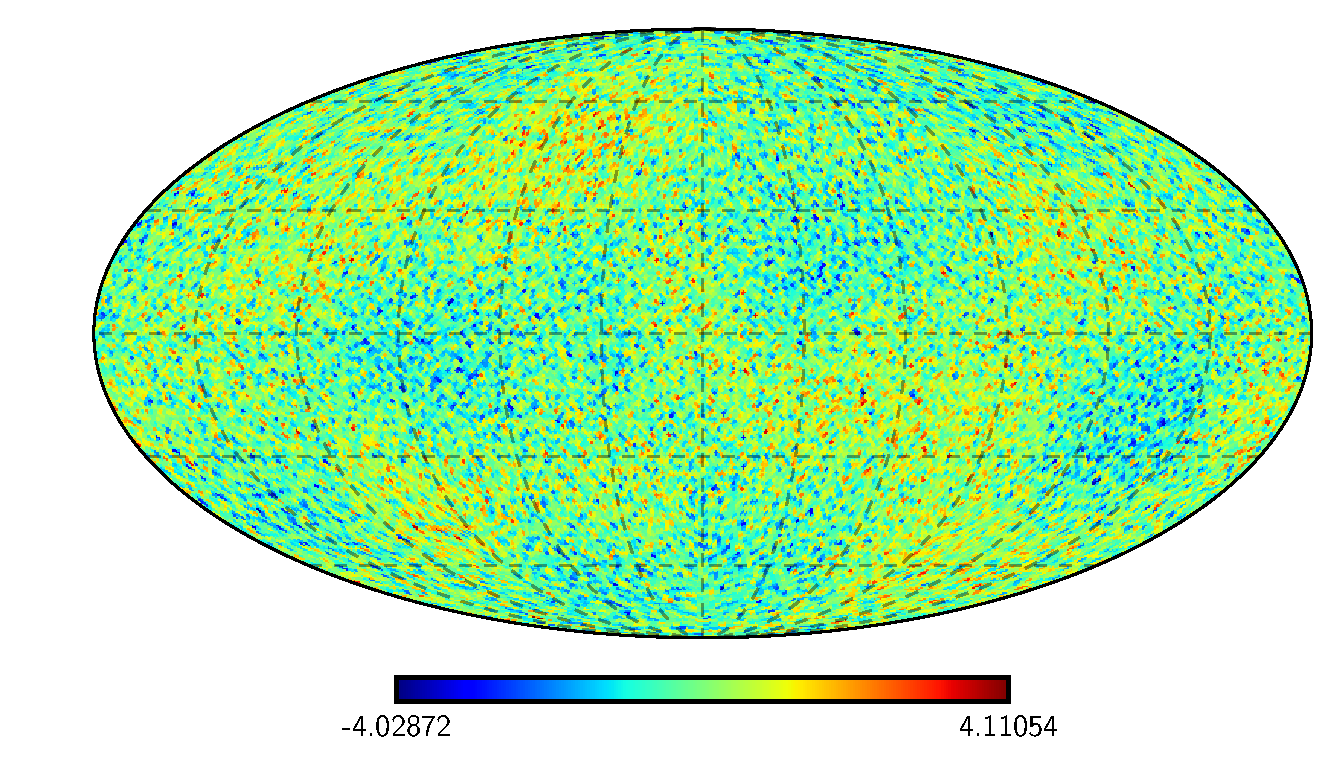
\includegraphics[width=0.31\columnwidth]{simulated/qu2eb/emap-healpix.pdf}}
\subfigure[E-mode local convolution]{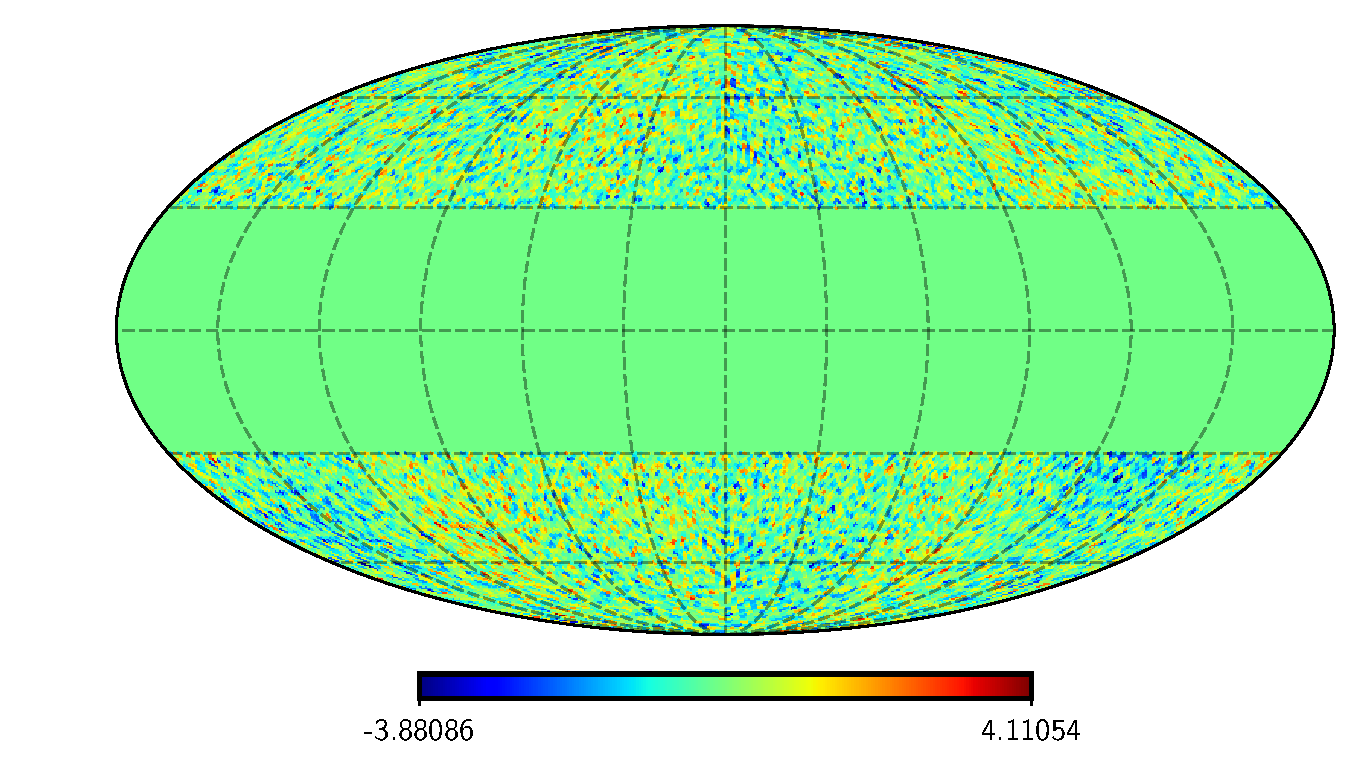
\includegraphics[width=0.31\columnwidth]{simulated/qu2eb/emap-2beta.pdf}}
\subfigure[Difference]{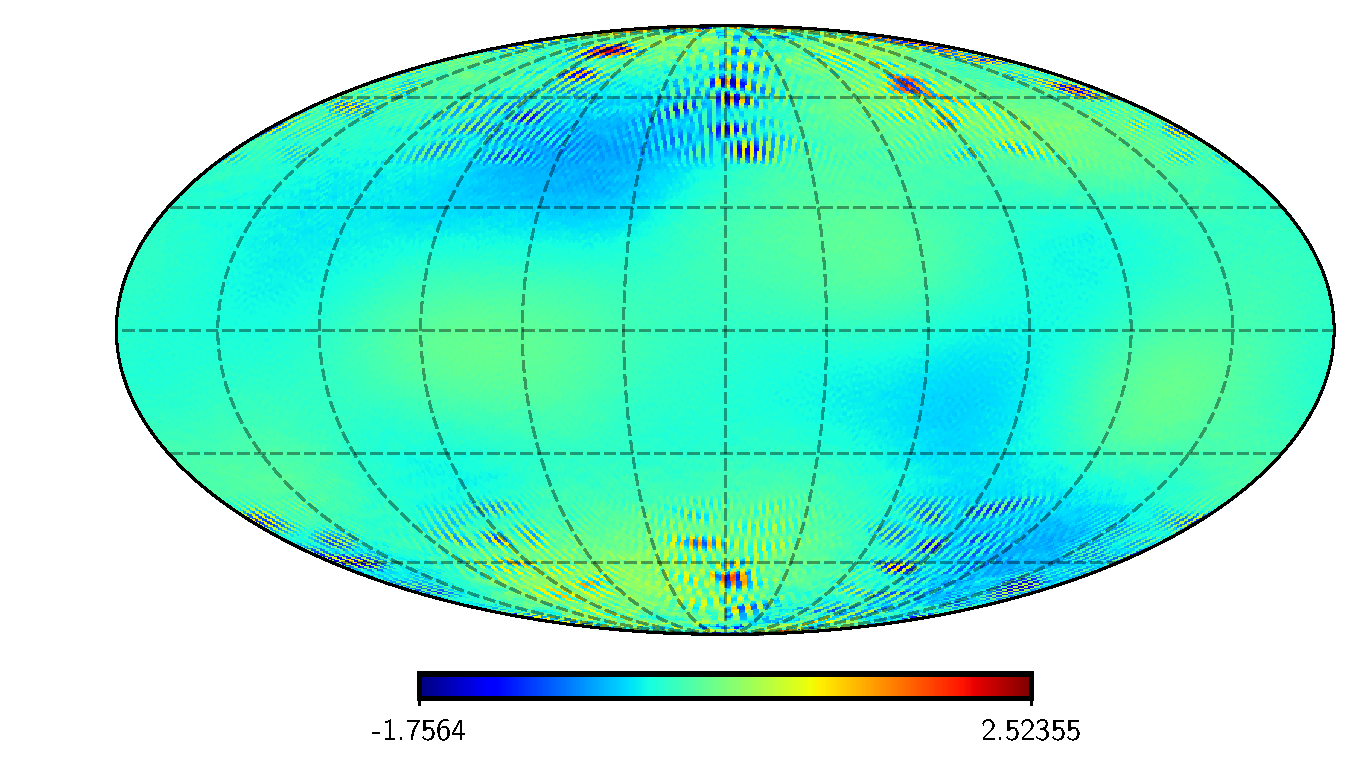
\includegraphics[width=0.31\columnwidth]{simulated/qu2eb/emap-diff.pdf}}
\subfigure[B-mode Healpix]{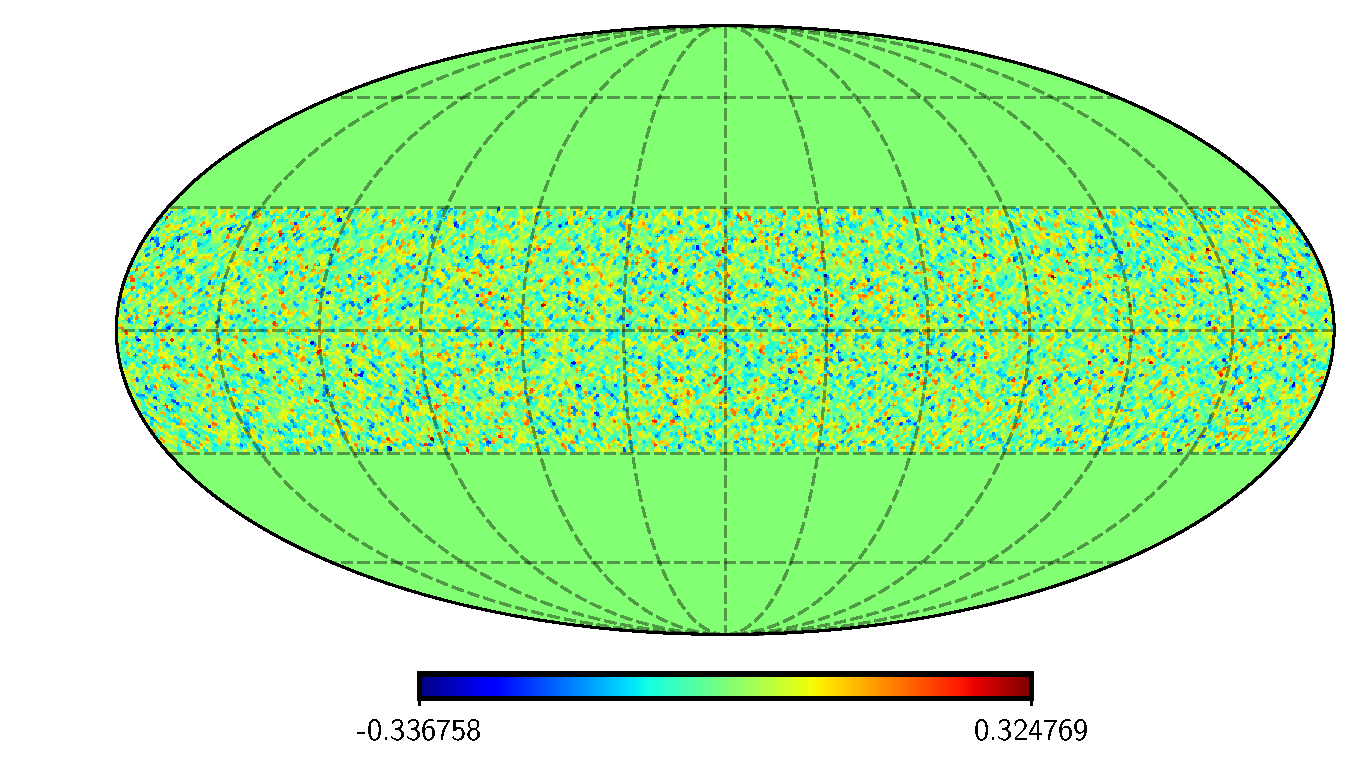
\includegraphics[width=0.31\columnwidth]{simulated/qu2eb/bmap-healpix.pdf}}
\subfigure[B-mode local convolution]{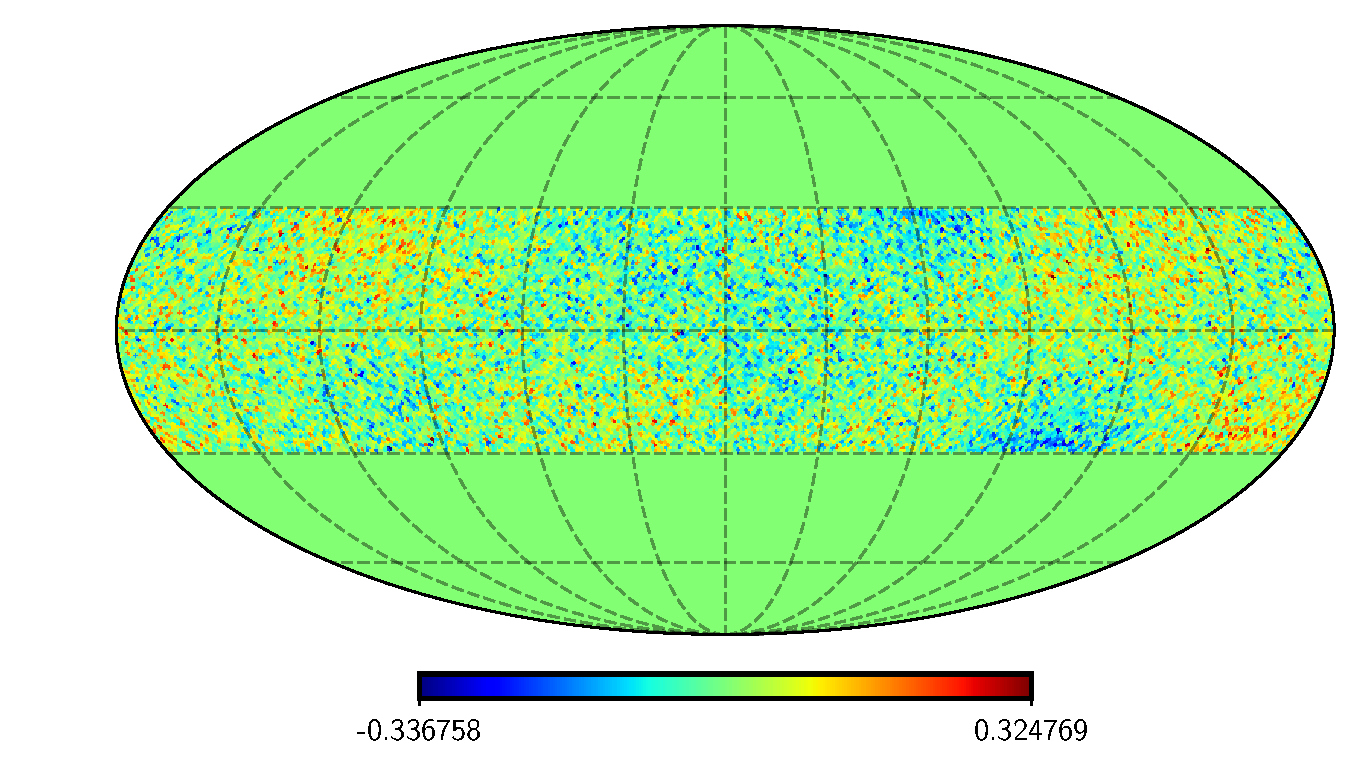
\includegraphics[width=0.31\columnwidth]{simulated/qu2eb/bmap-2beta.pdf}}
\subfigure[Difference]{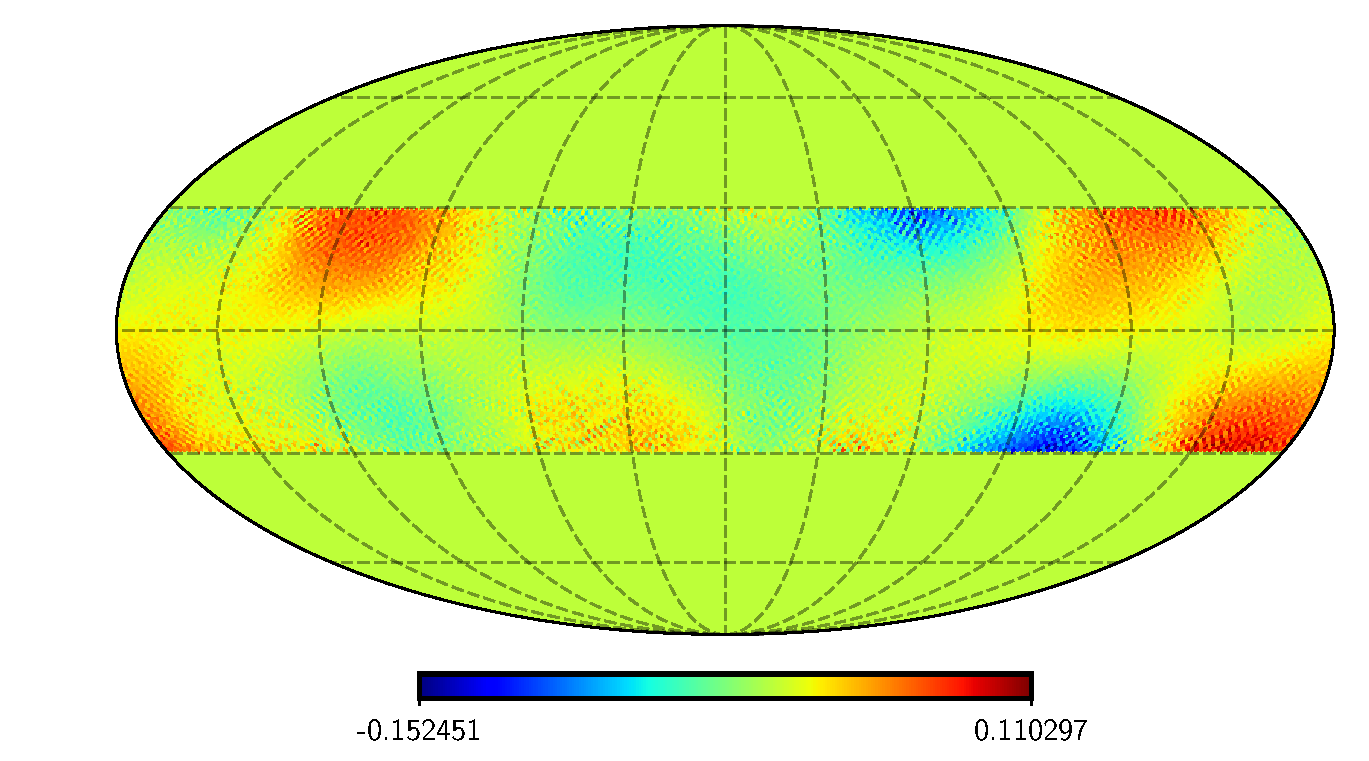
\includegraphics[width=0.31\columnwidth]{simulated/qu2eb/bmap-diff.pdf}}
\caption{{\textit Left:} Reference E \& B mode maps derived using Healpix. {\textit Middle:} E \& B mode maps derived using $r_{\rm cutoff}=2\beta_o$. The color scale is saturated to that of the respective reference maps. {\textit Right:} Difference between the maps shown in the left and middle columns.}
\label{fig:eb-maps-compare}
\end{figure}
%

Next we compute the power spectra of these local E \& B maps and compare them to the spectra derived from the reference maps. The results of this exercise are summarized in \fig{fig:eb-spectra_rad_cutoff}. We note that when the radial cutoff is set much below the non-locality parameter as in $r_{\rm cutoff}=0.25 \beta_o$, the spectra differ from the reference spectra by more the cosmic variance. However on increasing the radial cutoff to only $0.5\beta_o$, the differences at most multipoles reduce to being comparable to the cosmic variance. On further increasing the radial cutoff to $\beta_o$ and $2 \beta_o$, the difference at most multipoles further reduce to levels of 0.5 cosmic variance or in absolute terms the differences are at the level of 2\%. Also note that the improvement while transitioning from $r_{\rm cutoff}=\beta_o$ to $r_{\rm cutoff}=2 \beta_o$ are not as significant 
as seen while increasing the $r_{\rm cutoff}$ to $\beta_o$. This is can be understood as a consequence of the rapidly decaying nature of the radial kernels we discussed in \sec{sec:radial_locality}. 

At first glance, the above remarks seem to hold true only for the E mode spectra, since the errors in the B mode spectra seem to be significantly larger as seen in the middle row of \fig{fig:eb-spectra_rad_cutoff}. We understand that the higher error in the B mode spectra is primarily a combined effect of the low amplitude of the B mode spectrum as compared to the E mode spectrum and limited numerical accuracy of our simple convolution algorithm. We ran a number of tests to confirm these as reasons for the observed discrepant behaviour. 
%
\begin{figure}[!t] 
\centering
%\vspace{-5cm}
\subfigure[]{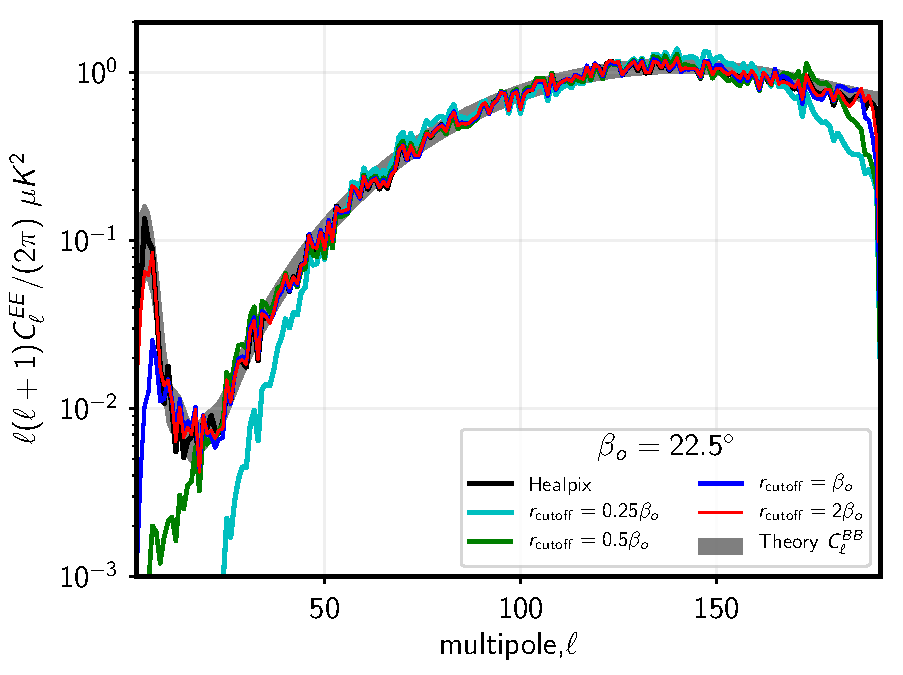
\includegraphics[width=0.49\columnwidth]{simulated/qu2eb/ee-spectrum-radial-cutoff.pdf}}
\subfigure[]{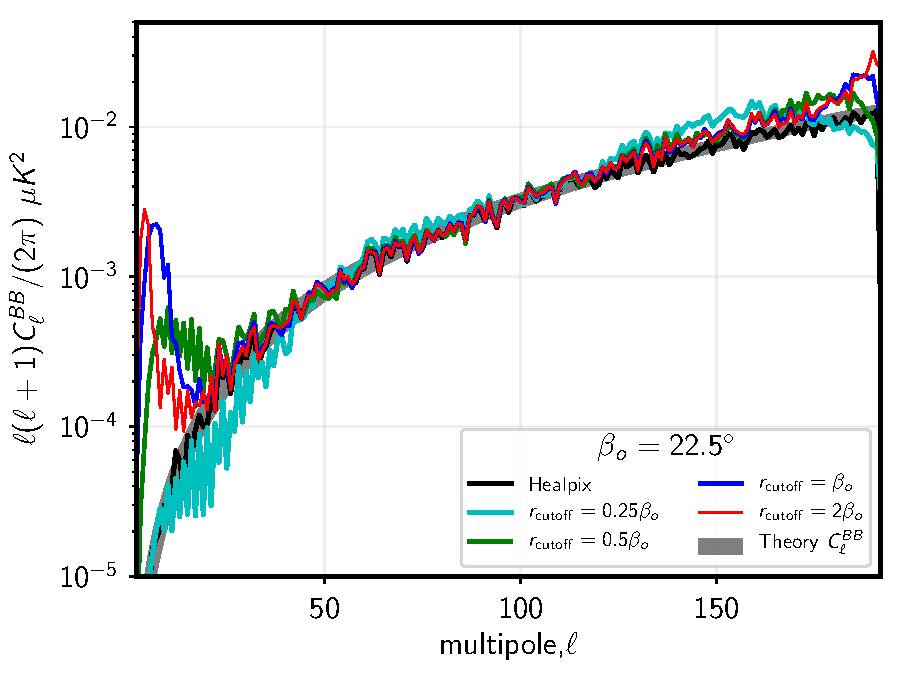
\includegraphics[width=0.49\columnwidth]{simulated/qu2eb/bb-spectrum-radial-cutoff.pdf}}\\[-6ex]
\subfigure[]{\includegraphics[width=0.49\columnwidth]{simulated/qu2eb/relative-percentage-err-ee-spectrum-radial-cutoff.pdf}}
\subfigure[]{\includegraphics[width=0.49\columnwidth]{simulated/qu2eb/relative-percentage-err-bb-spectrum-radial-cutoff.pdf}}\\[-6ex]
\subfigure[]{\includegraphics[width=0.49\columnwidth]{simulated/qu2eb/eqmask/relative-percentage-err-ee-spectrum-radial-cutoff.pdf}}
\subfigure[]{\includegraphics[width=0.49\columnwidth]{simulated/qu2eb/eqmask/relative-percentage-err-bb-spectrum-radial-cutoff.pdf}} \\[-2ex]
\caption{\textit{Top:} The figures on left and right depict the E mode spectra and the B mode spectra respectively. \textit{Middle:} These figures depict the relative percentage difference between the spectra derived from full sky, locally evaluated E \& B  maps and the reference spectra. \textit{Bottom:} These figures depict the same results as shown in the middle row, except that the regions with $|b|>30^\circ$ of the maps have been masked for this analysis. 
The colors indicate the spectra derived from imposing different radial cutoff as indicated by the legends. The gray bands indicate the cosmic variance scatter around the fiducial spectra. The dashed horizontal black lines mark the 2\% error.}
\label{fig:eb-spectra_rad_cutoff}
\end{figure}
%
We exchanged the E and B mode spectra, \revisit{(taking care to set $C_{\ell}^{TE}=0$)} and noted that the trends observed in the error plots are reversed, clearly indicating a dependence on the amplitude of the spectrum. We noted that the polar caps were particularly error prone, as seen in \fig{fig:eb-maps-compare}. We excised these error prone regions, specifically masking portions of the maps with $|b|>30^{\circ}$ to find that the errors on the B mode spectra revert to having very similar structure as that of the E mode spectra, as seen in the bottom row of \fig{fig:eb-spectra_rad_cutoff}. Finally we modify the use of standard Healpix routines to mimic the local convolution E \& B construction (see \app{sec:convolution_err} for details). The results from this exercise also concur with our understanding of the discrepant behaviour for the B-mode spectrum.
%--------------------------------------------------------
%--------------------------------------------------------
\subsection{Separating Stokes Q \& U maps corresponding to E \& B modes of polarization}
In this section we present the results of evaluating the local convolution given in \eq{eq:op_qu2equbqu}, to decompose the total Stokes Q and U parameters into those correspond to the E modes and B modes of polarization respectively. We reiterate that this procedure uses real space operation on the total Stokes Q and U maps and does not go through the process of constructing the E and B modes as is usually the case. 
%
\begin{figure}[!t] 
\centering
\subfigure[E Q-map: Healpix]{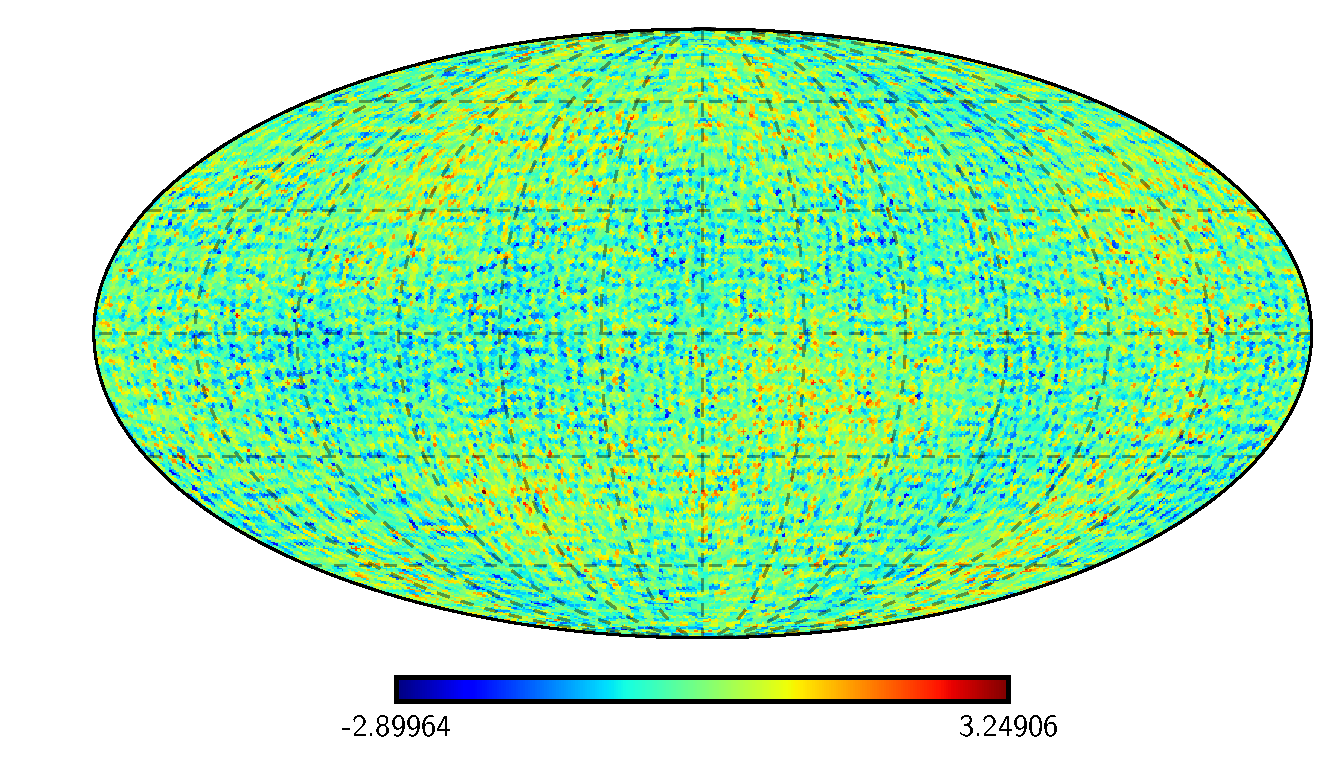
\includegraphics[width=0.31\columnwidth]{simulated/qu2equbqu/e-qmap-healpix.pdf}}
\subfigure[E Q-map: Local convolution]{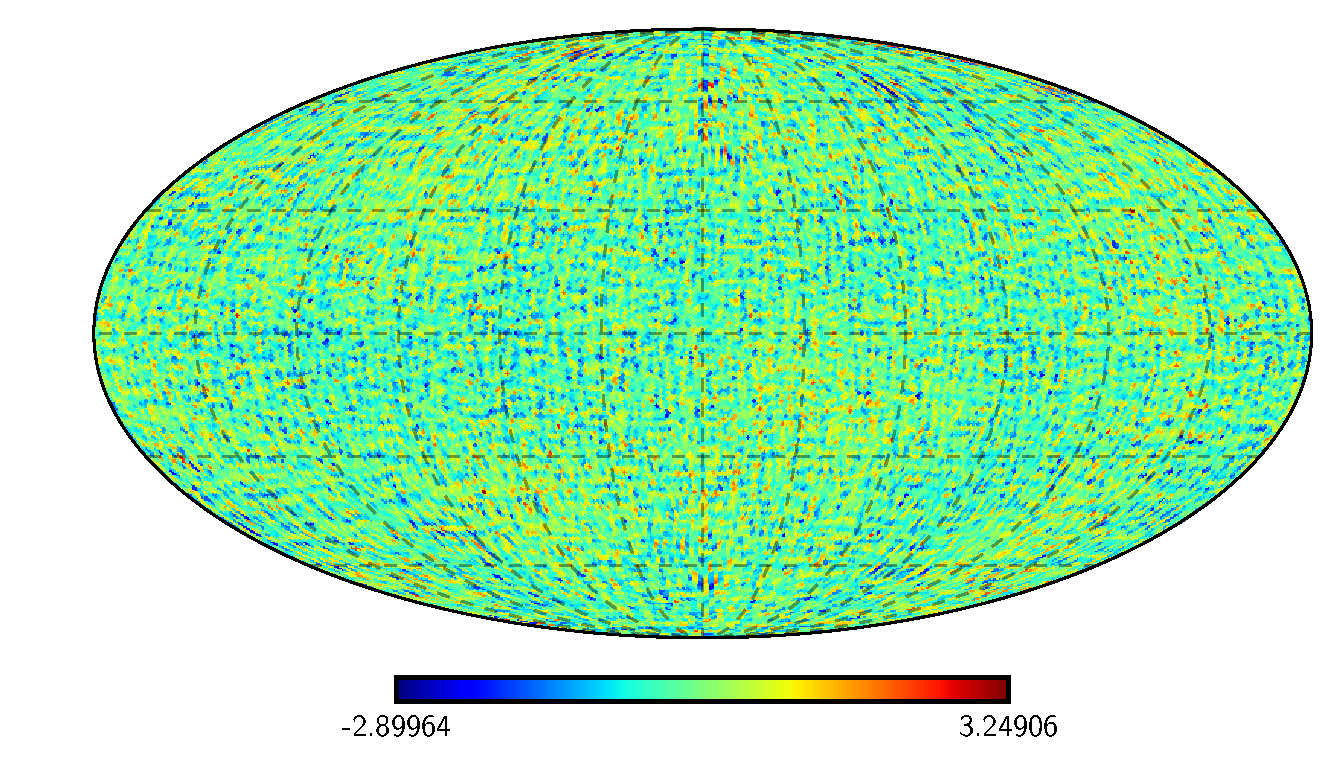
\includegraphics[width=0.31\columnwidth]{simulated/qu2equbqu/e-qmap-2beta.pdf}}
\subfigure[E Q-map: Difference]{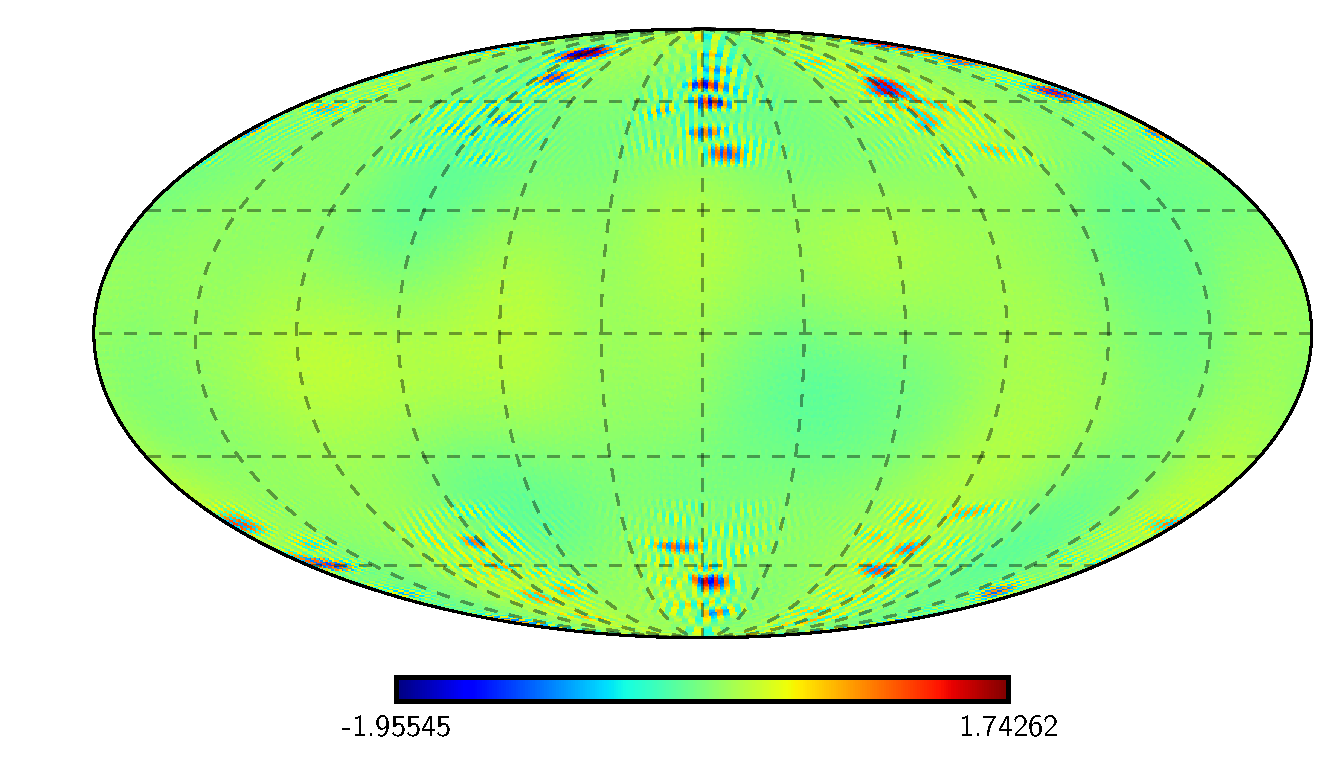
\includegraphics[width=0.31\columnwidth]{simulated/qu2equbqu/e-qmap-diff.pdf}}
\subfigure[E U-map: Healpix]{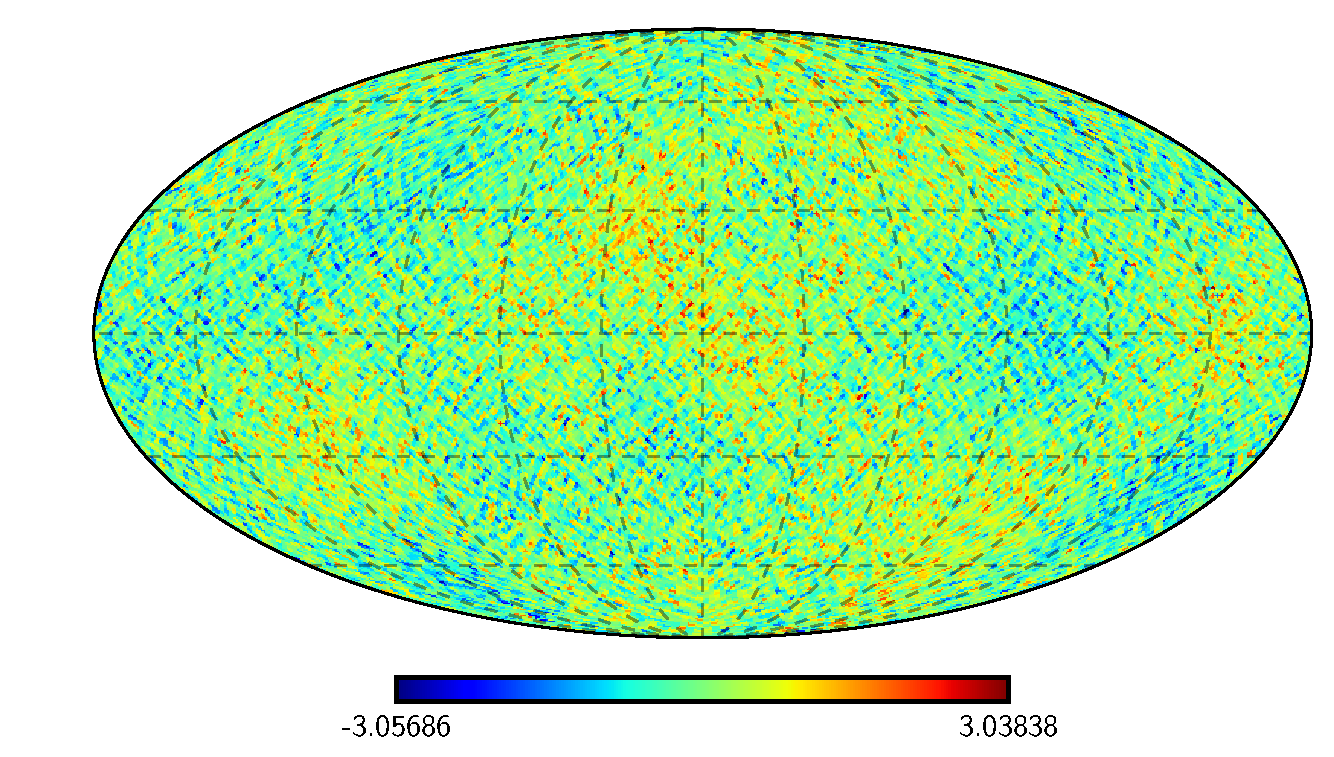
\includegraphics[width=0.31\columnwidth]{simulated/qu2equbqu/e-umap-healpix.pdf}}
\subfigure[E U-map: Local convolution]{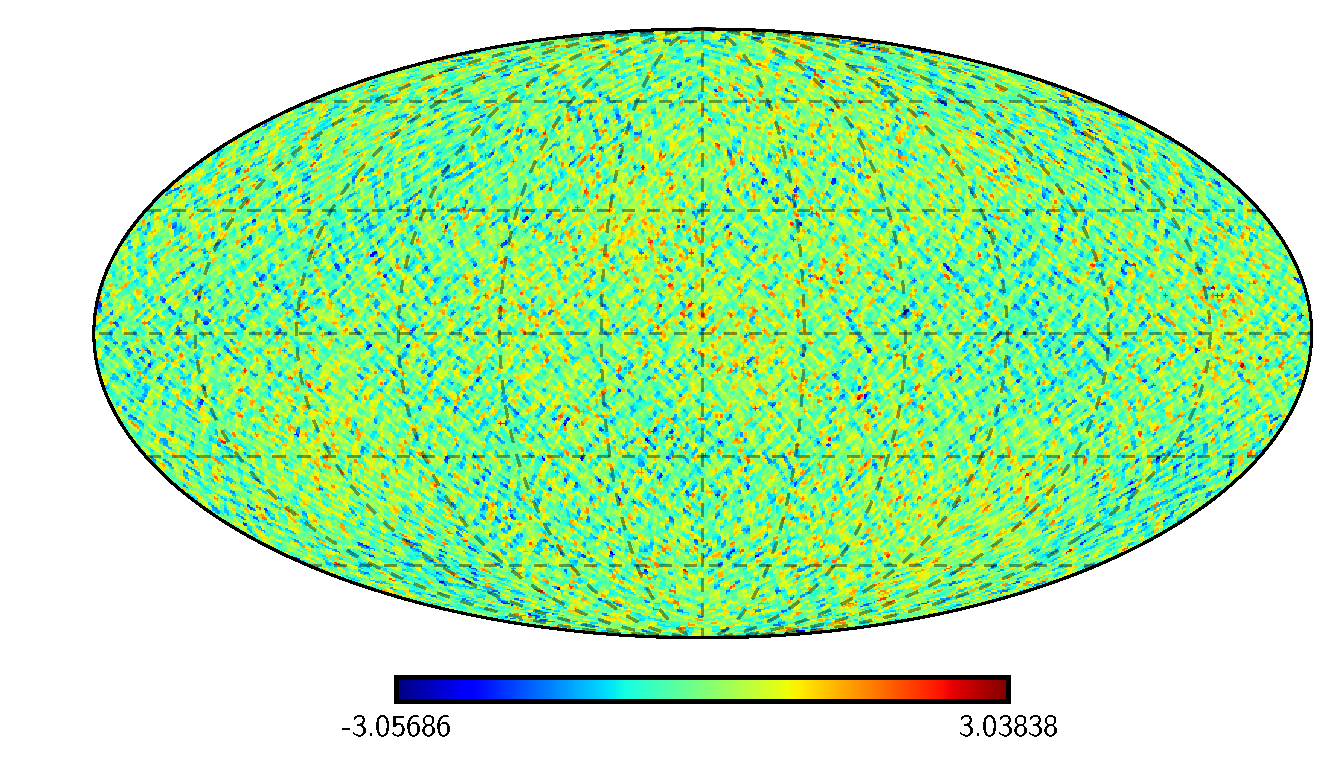
\includegraphics[width=0.31\columnwidth]{simulated/qu2equbqu/e-umap-2beta.pdf}}
\subfigure[E U-map: Difference]{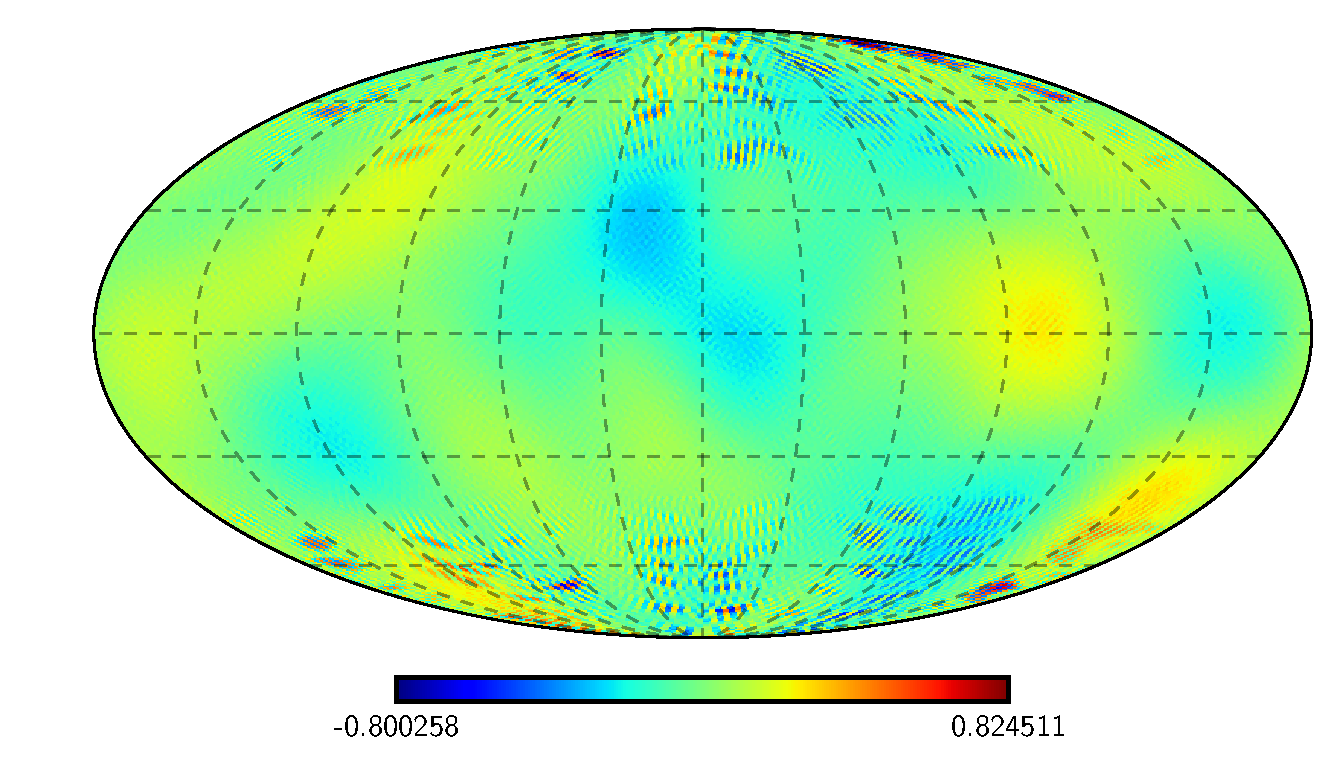
\includegraphics[width=0.31\columnwidth]{simulated/qu2equbqu/e-umap-diff.pdf}}
\subfigure[B Q-map: Healpix]{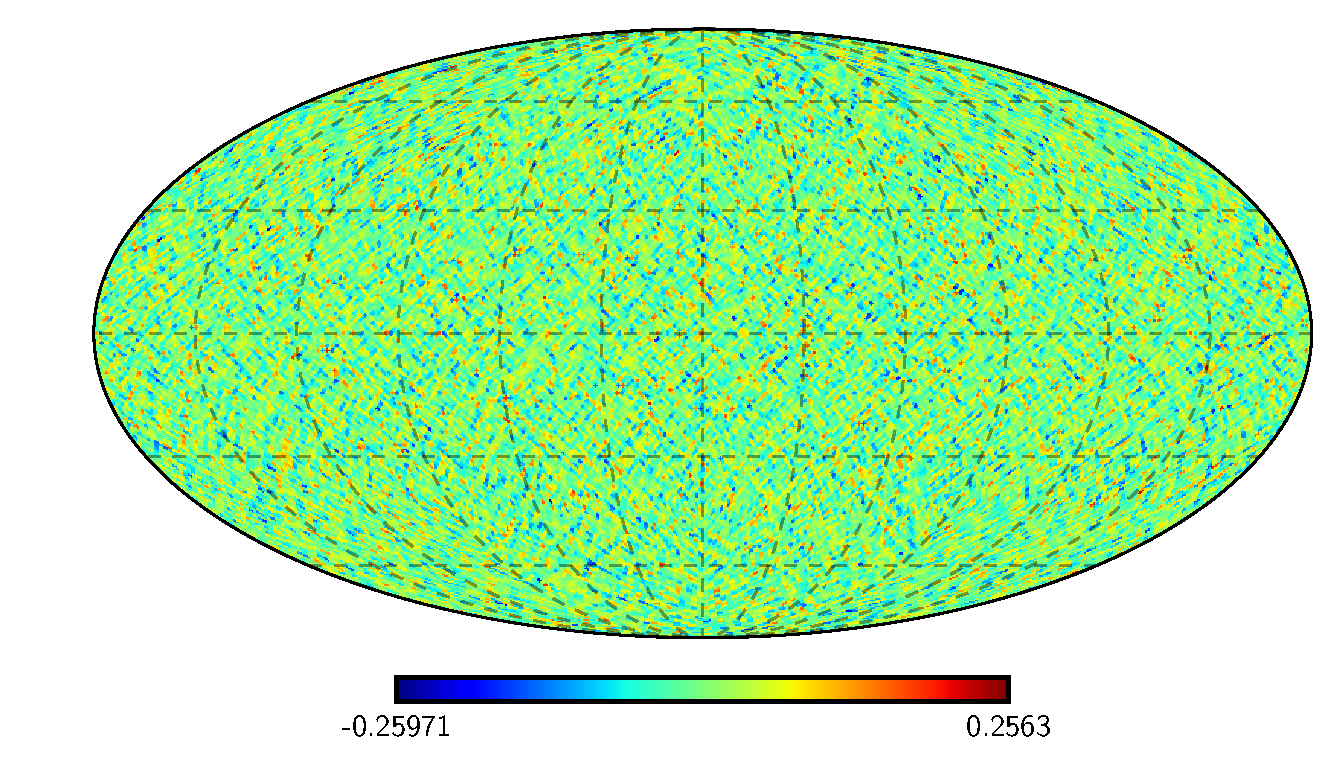
\includegraphics[width=0.31\columnwidth]{simulated/qu2equbqu/b-qmap-healpix.pdf}}
\subfigure[B Q-map: Local convolution]{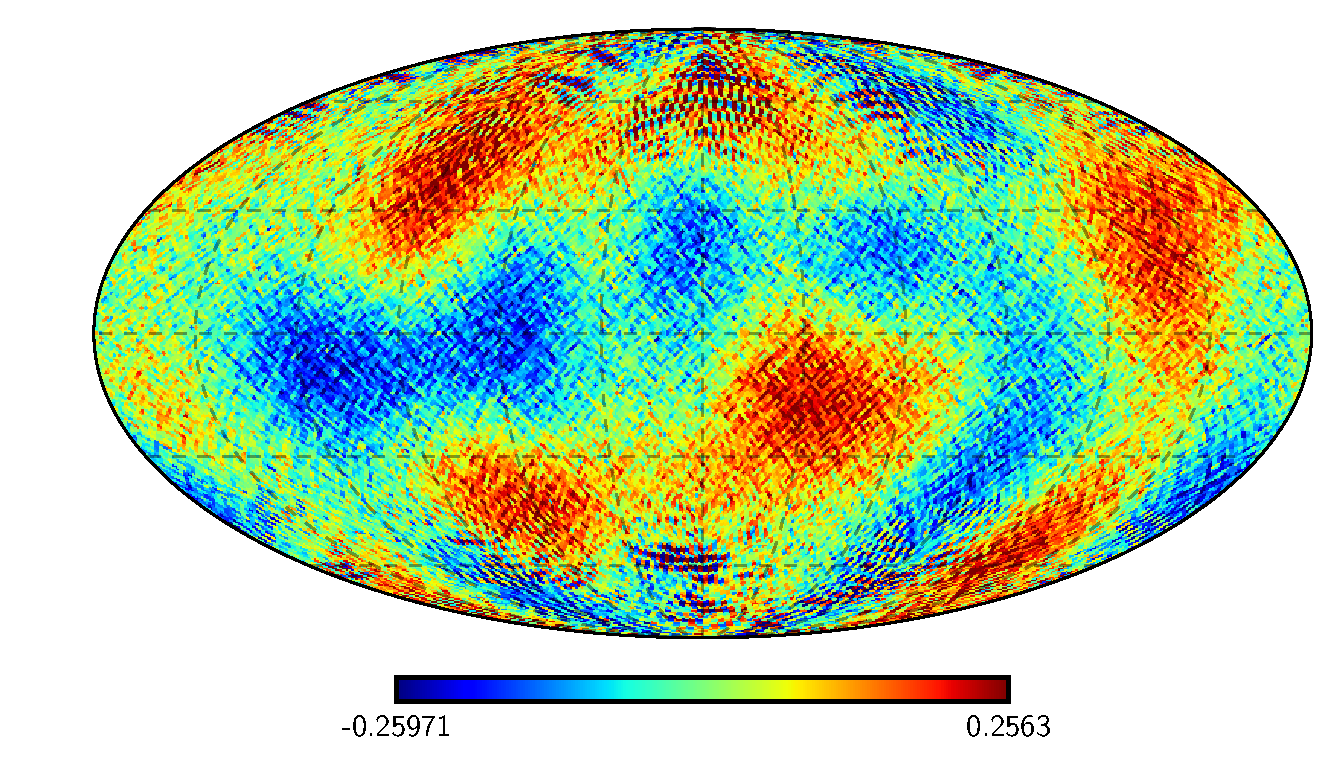
\includegraphics[width=0.31\columnwidth]{simulated/qu2equbqu/b-qmap-2beta.pdf}}
\subfigure[B Q-map: Difference]{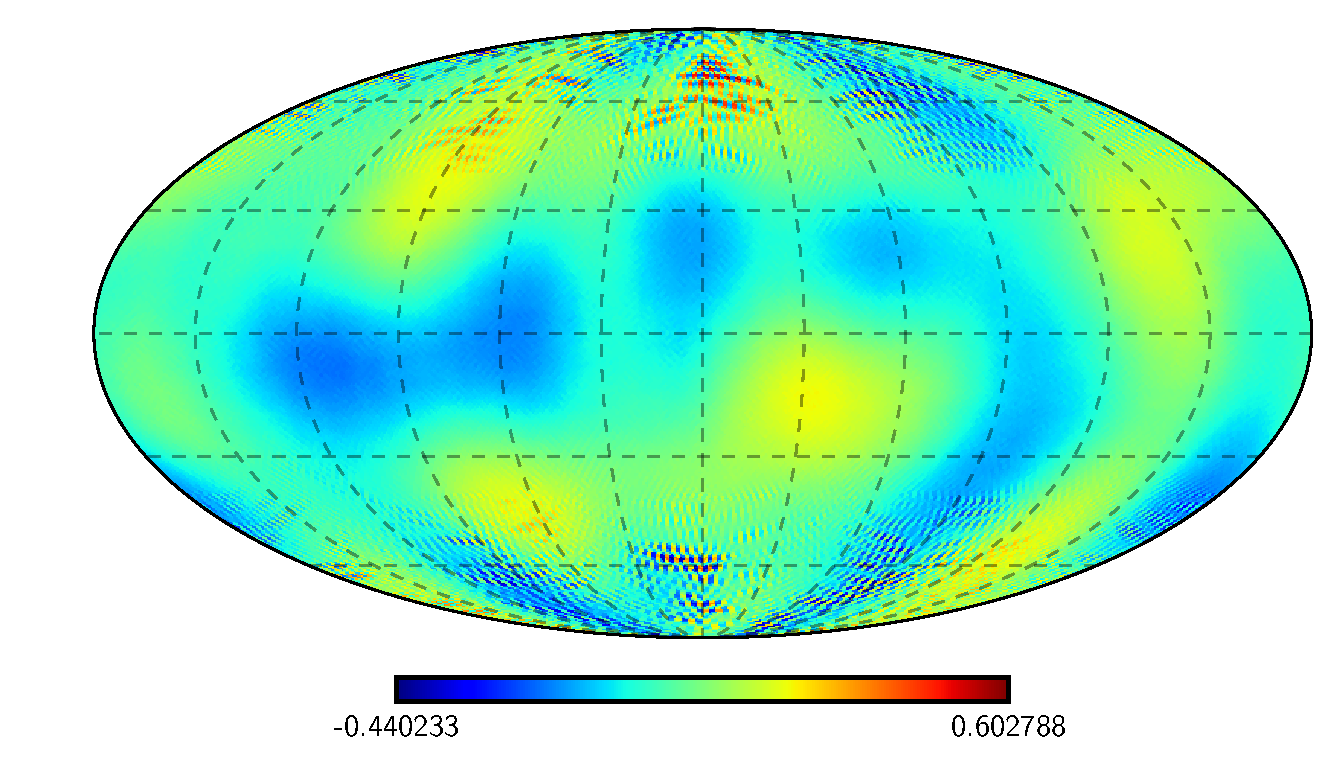
\includegraphics[width=0.31\columnwidth]{simulated/qu2equbqu/b-qmap-diff.pdf}}
\subfigure[B U-map: Healpix]{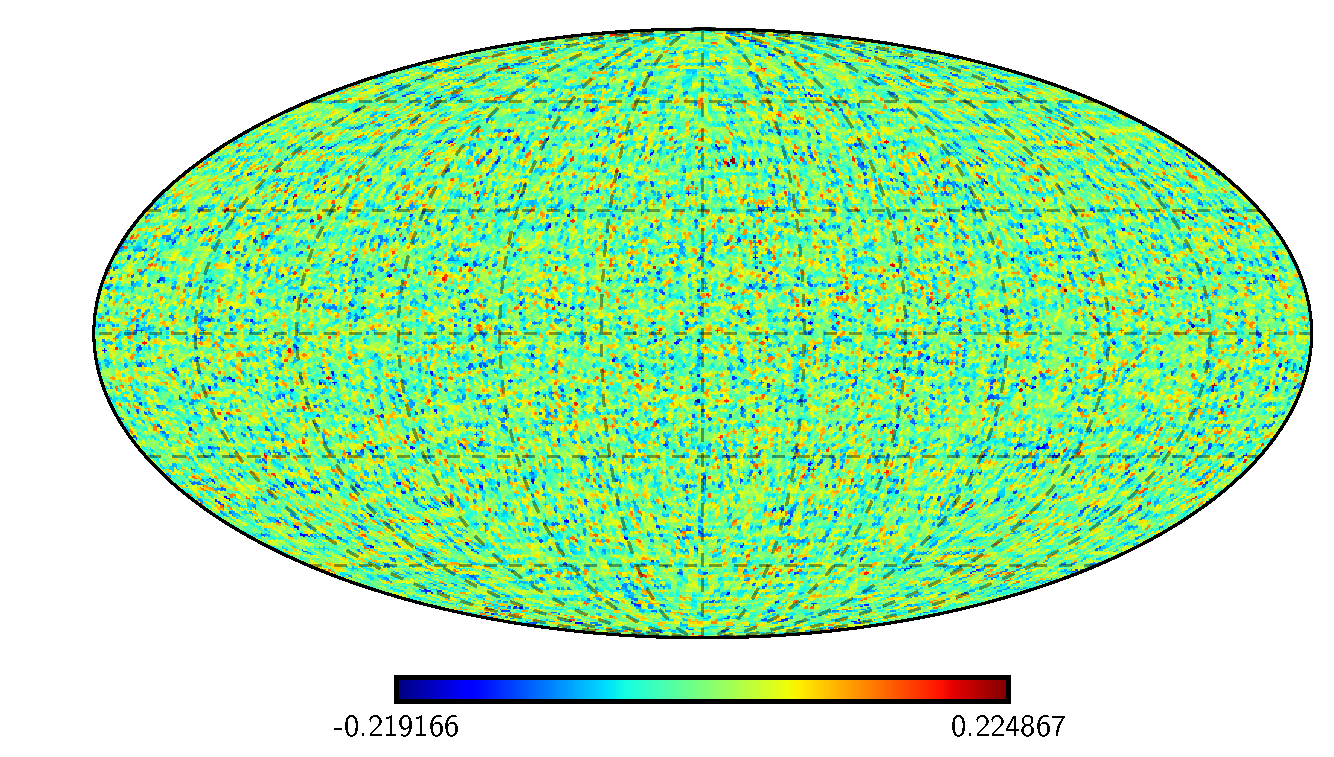
\includegraphics[width=0.31\columnwidth]{simulated/qu2equbqu/b-umap-healpix.pdf}}
\subfigure[B U-map: Local convolution]{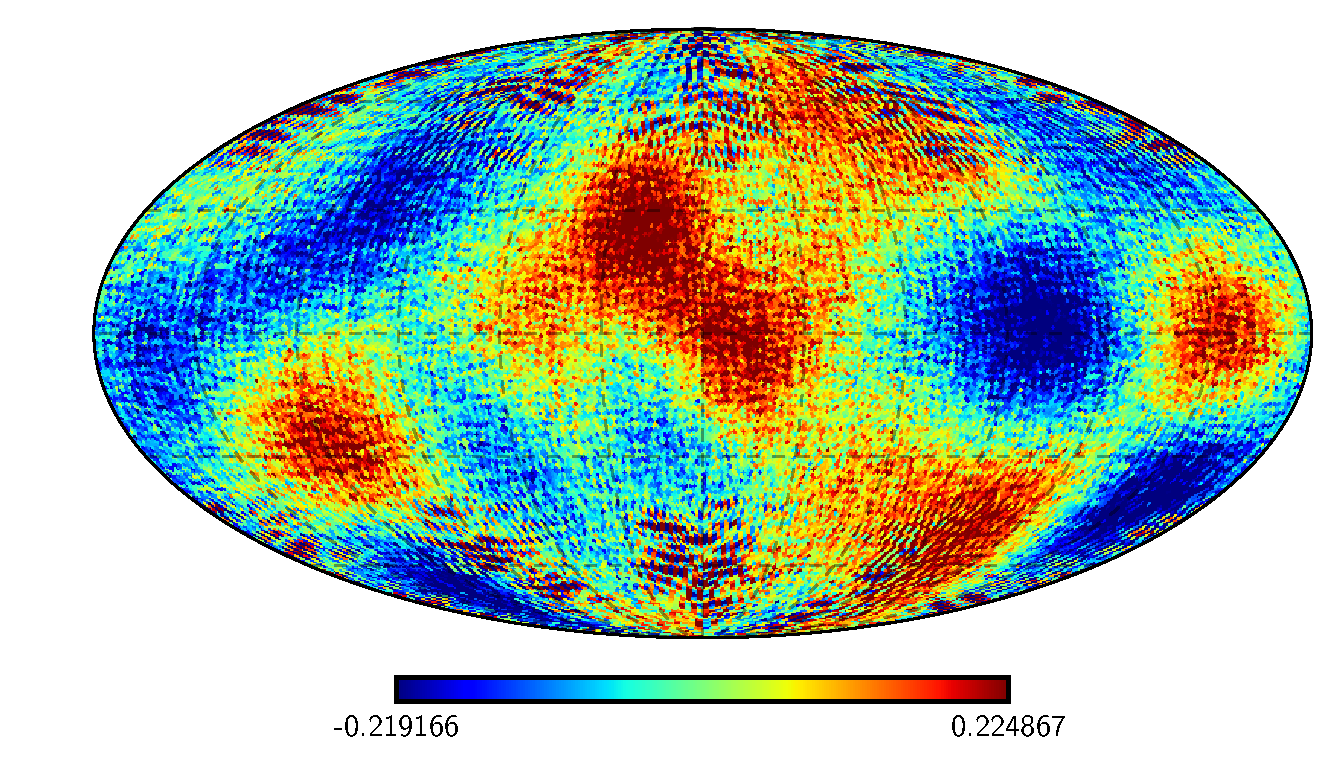
\includegraphics[width=0.31\columnwidth]{simulated/qu2equbqu/b-umap-2beta.pdf}}
\subfigure[B U-map: Difference]{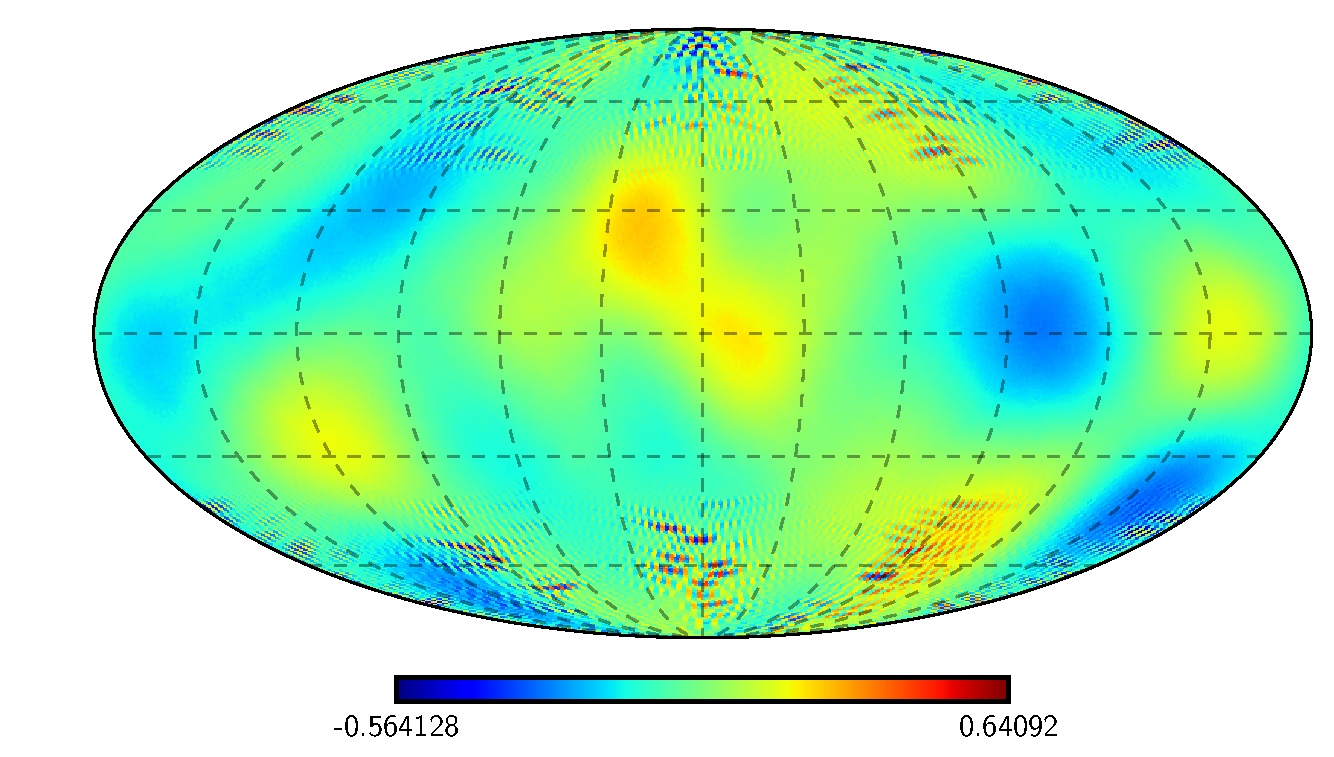
\includegraphics[width=0.31\columnwidth]{simulated/qu2equbqu/b-umap-diff.pdf}}
\caption{The top two rows depict the Stokes Q \& U maps  respectively corresponding to E mode of polarization while the bottom two rows depict  the Stokes Q \& U maps  respectively corresponding to the  B modes of polarization. \textit{Left:} Stokes Maps derived using Healpix. \textit{Middle}: Stokes maps derived using local convolution with $r_{\rm cutoff} = 2 \beta_o$. \textit{Right:} Difference between the maps derived using the two different methods.}
\label{fig:equ-bqu-maps-compare}
\end{figure}
%
The resultant Stokes Q and U maps corresponding to the E mode are depicted in the first two rows while those corresponding to B modes are shown in the final two rows of \fig{fig:equ-bqu-maps-compare}.  The local convolution maps depicted in this figure are computed using a radial cutoff of $r_{\rm cutoff }=2\beta_o$. Note that similar to observations of the previous section, the maps derived via local real space convolutions, suffer from having relatively higher error in the polar caps, while the differences in the  band around the equator are smaller and dominated by large scale modes.
%
\begin{figure}[!t] 
\centering
\subfigure[]{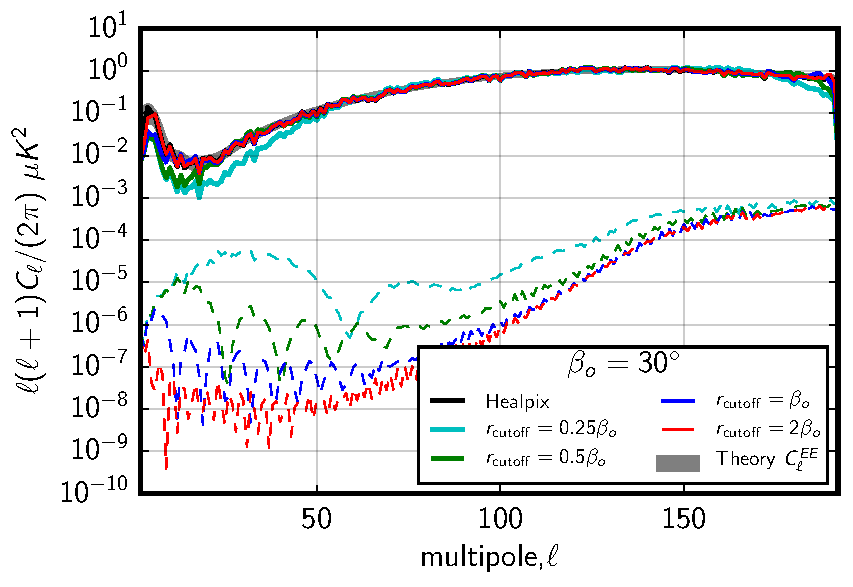
\includegraphics[width=0.49\columnwidth]{simulated/qu2equbqu/equ-spectra-radial-cutoff.pdf}}
\subfigure[]{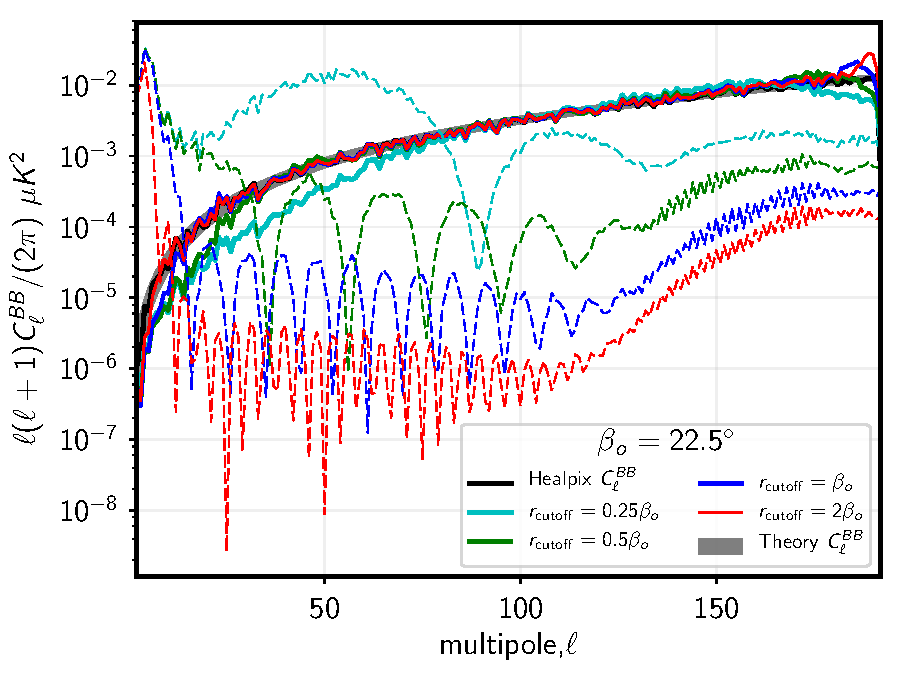
\includegraphics[width=0.49\columnwidth]{simulated/qu2equbqu/bqu-spectra-radial-cutoff.pdf}}\\[-5ex]
\subfigure[]{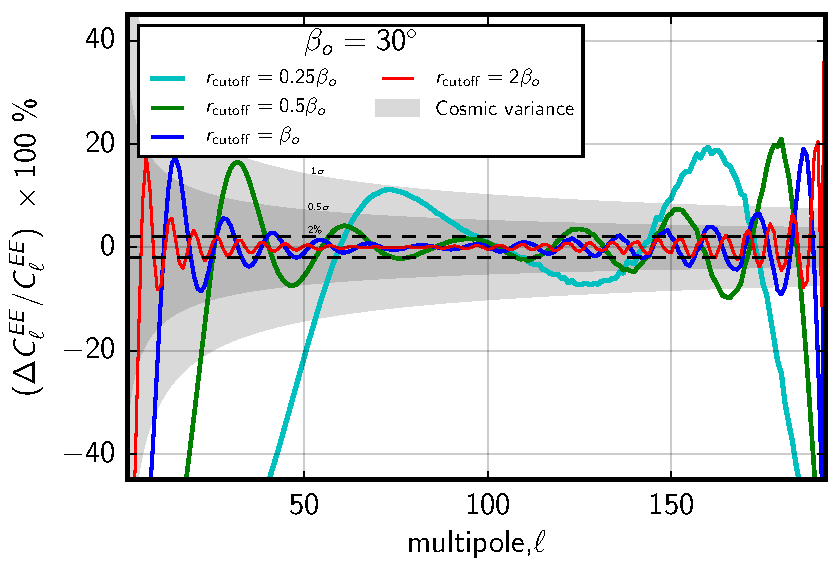
\includegraphics[width=0.49\columnwidth]{simulated/qu2equbqu/relative-percentage-err-equ-e-spectrum-radial-cutoff.pdf}}
\subfigure[]{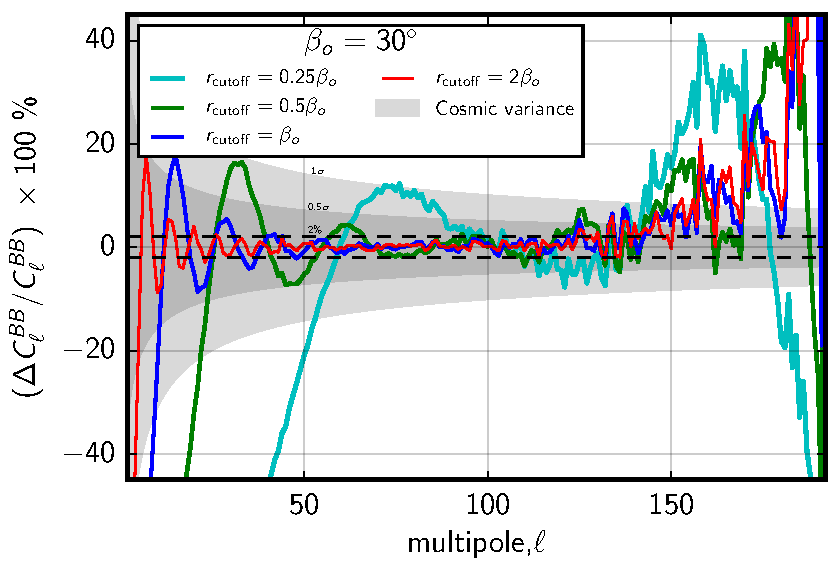
\includegraphics[width=0.49\columnwidth]{simulated/qu2equbqu/relative-percentage-err-bqu-b-spectrum-radial-cutoff.pdf}}
\caption{\textit{Top:} The thick lines in the figure on left depicts the E mode spectra derived from pure E Stokes Q and U maps derived using different radial cutoffs, while the thin lines depict the residual B mode power. The figure on the right depict the same except that the thick lines now depict the B mode spectra while the thin lines show the residual E mode power. \textit{Bottom:} The figure on the left and right depict the difference between the reference spectra and those derived from local convolution maps for different $r_{\rm cutoff}$ imposed on the convolution. In all the panels the color of the lines indicate the radial cutoff as indicated by the legend and the gray band marks the cosmic variance around the fiducial spectra.}
\label{fig:equ-bqu-spectra_rad_cutoff}
\end{figure}
%
Next we compute the E and B mode spectra from the set of Stokes maps constructed using local convolutions with different $r_{\rm cutoff}$. Note that for this exercise we use the standard Healpix routines for computing the spectra from the Stokes maps. The spectra derived from these local convolution maps and their difference with respect to the reference spectra are depicted in \fig{fig:equ-bqu-spectra_rad_cutoff}. The observations are similar to that made in the previous section: the difference with respect to the reference spectra reduce on increasing the radial cutoff and reach 2\% levels at most multipoles for the maximum radial $r_{\rm cutoff} =2 \beta_o$ used in this analysis.
In particular here we note that the B-mode residue in the Stokes Q \& U maps corresponding to E-modes is much smaller as compared to the E-mode residue in the Stokes Q \& U maps  computed for the B-modes of polarization. At all multipoles the B-mode residual power is below the lensing B-modes. The E-mode residual power at low multipoles is almost fully intact. 

Motivated by these observations we also compute the Stokes Q \& U maps corresponding to B-modes of polarization by simply subtracting the Stokes Q \& U maps corresponding to E-mode from the total Stoker Q \& U maps. For completeness we also compute the Stokes Q \& U maps corresponding to E-mode in an analogous manner. We carry out a spectral study on these Stokes Q \& U maps corresponding to E \& B modes, computed using this alternate method. The results of the spectral analysis are summarized in \fig{fig:dbqu-spectra_rad_cutoff}.
%
\begin{figure}[!t] 
\centering
%\subfigure[]{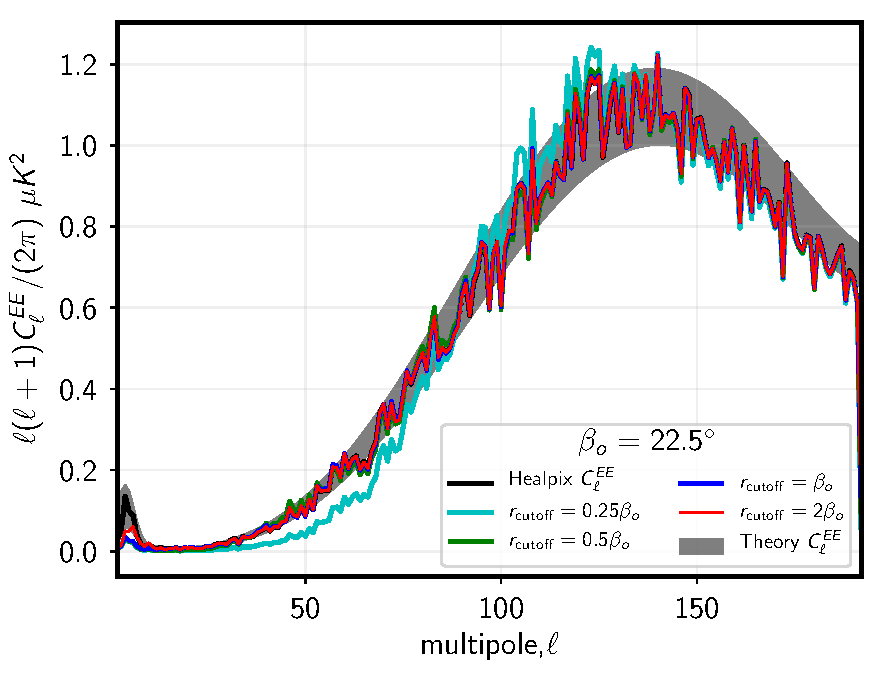
\includegraphics[width=0.49\columnwidth]{simulated/qu2equbqu/dequ-spectra-radial-cutoff.pdf}}
%\subfigure[]{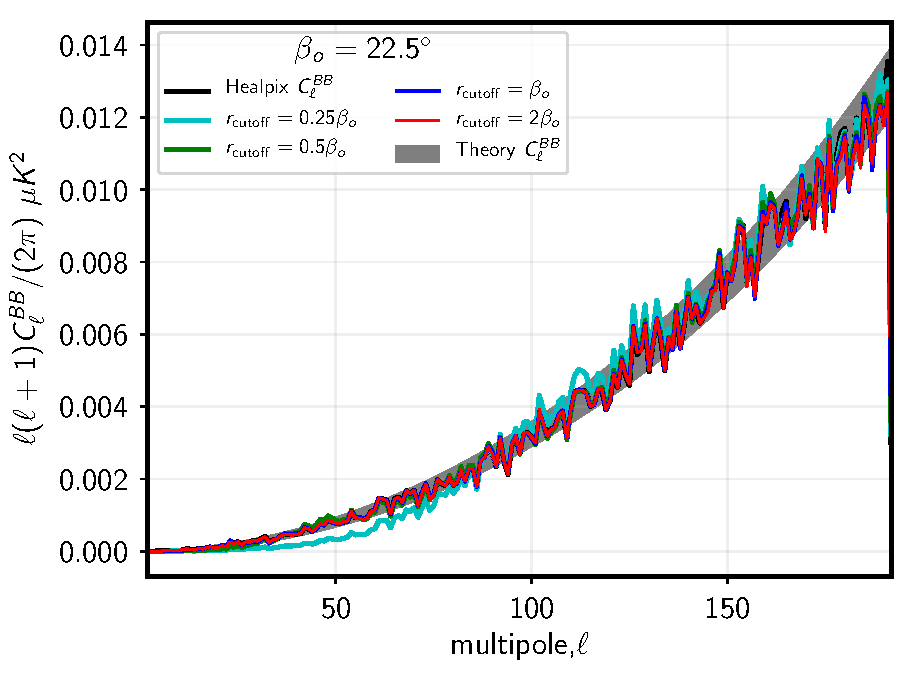
\includegraphics[width=0.49\columnwidth]{simulated/qu2equbqu/dbqu-spectra-radial-cutoff.pdf}} \\[-5ex]
\subfigure[]{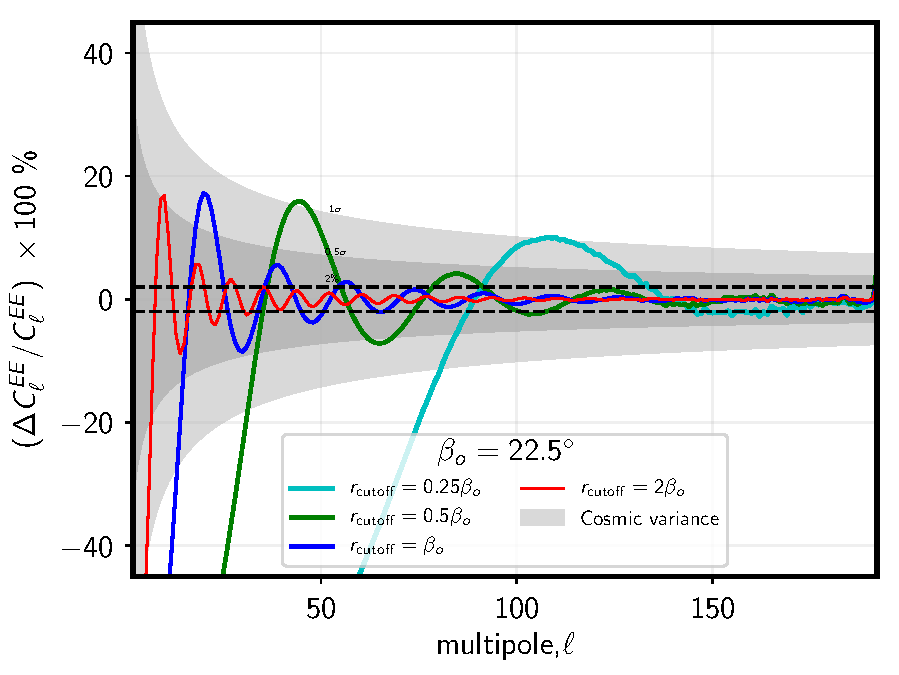
\includegraphics[width=0.49\columnwidth]{simulated/qu2equbqu/relative-percentage-err-equ-de-spectrum-radial-cutoff.pdf}}
\subfigure[]{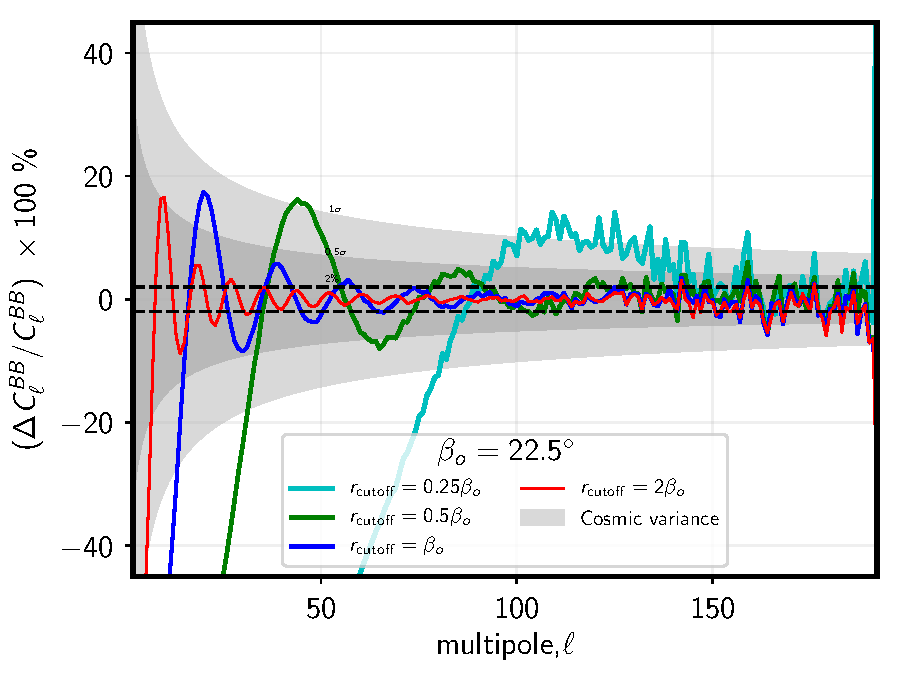
\includegraphics[width=0.49\columnwidth]{simulated/qu2equbqu/relative-percentage-err-bqu-db-spectrum-radial-cutoff.pdf}}
\caption{This figure depicts the same as the bottom panel of \fig{fig:equ-bqu-spectra_rad_cutoff}. The Stokes Q and U maps corresponding to E and B modes used in this analysis are constructed using the following relations:  $[Q,U]_{E}=[Q,U]-[Q,U]_{Local}^B$ ; $[Q,U]_{B}=[Q,U]-[Q,U]_{Local}^{E}$.}
\label{fig:dbqu-spectra_rad_cutoff}
\end{figure}
%
We observe that the the low multipole spectral behavior is not affected by this alternate construction of pure Stokes Q \& U maps. The high multipole behavior is significantly altered as can be seen by comparing \fig{fig:dbqu-spectra_rad_cutoff} with lower panels of \fig{fig:equ-bqu-spectra_rad_cutoff}. The relative percentage difference with respect to the reference spectra is seen to lie well within 2\% error for sufficiently high multipoles for all radial cutoff $r_{\rm cutoff}$.
%--------------------------------------------------------
%--------------------------------------------------------
\subsection{Multipole filtering using spatial convolutions}
 In this section we construct radial kernels which result in the desired multipole filtering, which can be achieved by simply controlling the $\ell_{\rm min}$ \& $\ell_{\rm max}$ arguments of the functions $f(\beta,\ell_{\rm min},\ell_{\rm max})$ and ${}_{\pm 2}f(\beta,\ell_{\rm min},\ell_{\rm max})$. \revisit{We reiterate that only the radial part of the convolution kernel encodes the multipole information, while the azimuthal part of the kernel is independent of multipoles. As seen in the previous sections, using local convolution methods to separate E and B modes does not allow the recovery of large scale modes. 
 %
\begin{figure}[!t]
\centering
\subfigure[]{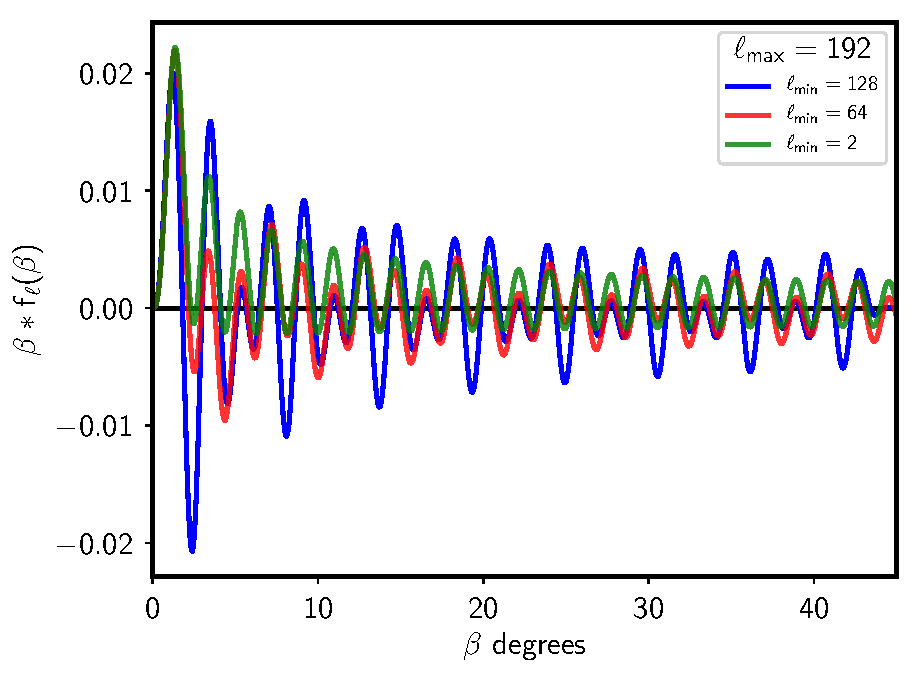
\includegraphics[width=1.\columnwidth]{simulated/multipole_filter/f_rad_ker_fn_vary_lmin.pdf}}\\
\subfigure[]{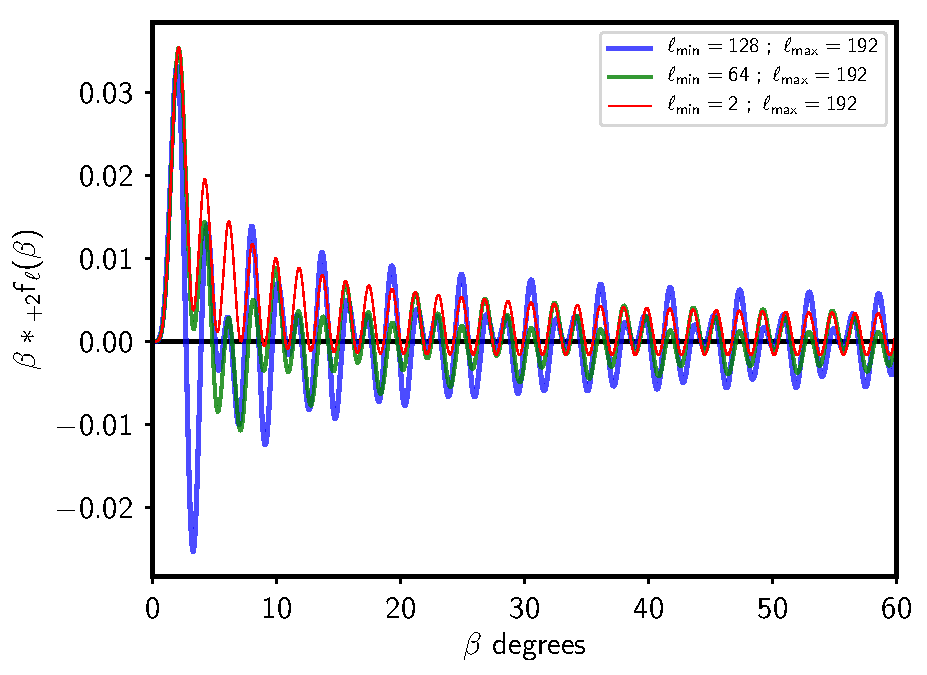
\includegraphics[width=0.48\columnwidth]{simulated/multipole_filter/fp2_rad_ker_fn_vary_lmin.pdf}}
\subfigure[]{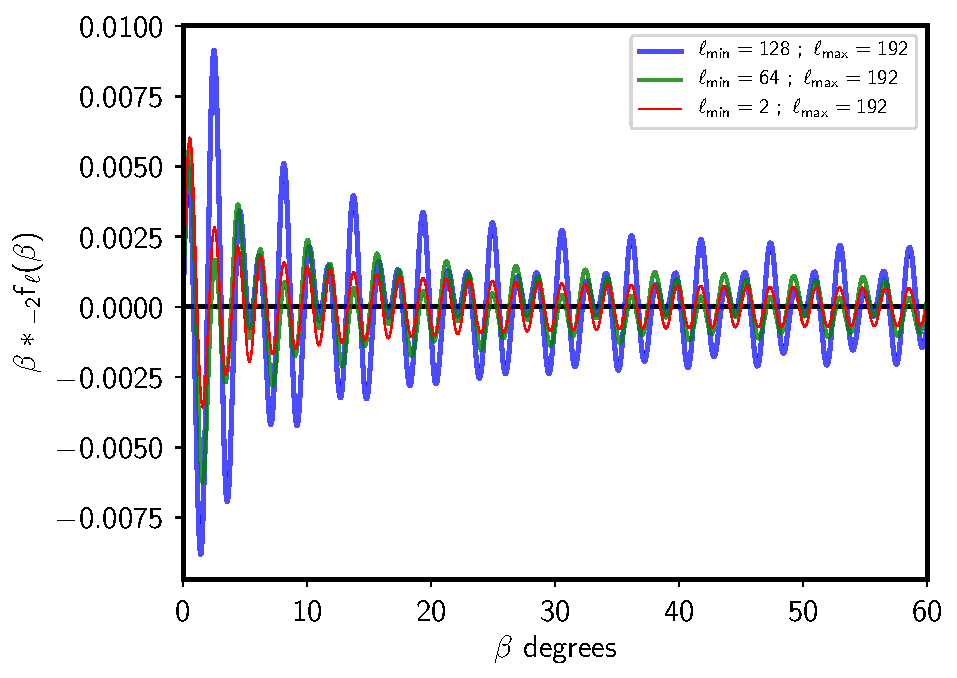
\includegraphics[width=0.48\columnwidth]{simulated/multipole_filter/fm2_rad_ker_fn_vary_lmin.pdf}}
\caption{This figure depicts the all the radial kernels evaluated for different multipole filters. In the filtered kernels presented here, only $\ell_{\rm min}$ has been altered while the maximum multipole is held fixed at $\ell_{\rm max}=192$. The kernels have been multiplied by a factor of the argument $\beta$ to highlight the differences in the kernel at large angular separations $\beta$.}
\label{fig:rad_ker_multipole_filter}
\end{figure}
%
This can be understood as occurring due to the following reason: localizing the convolution kernel by introducing a radial cut off, progressively reduces the overlap of the kernels for pixels on increasing the separation between them. The overlap begins to significantly drop when angular distances are larger than $r_{\rm cutoff}$ and reaches a null at a separation of  $2 r_{\rm cutoff}$. Owing to this overlap reduction, the pixels at large separation in the constructed maps have a reduced correlation, specifically $C(\theta > 2 r_{\rm cutoff})=0$.}  This motivates the construction of high pass filters especially while working with local convolution maps. \comment{This should results in systematically lower power on large angular scales. This is observed for E mode spectra, but not quiet for B. Why is that ?}.  
%
\begin{figure}[!t]
\centering
\subfigure[]{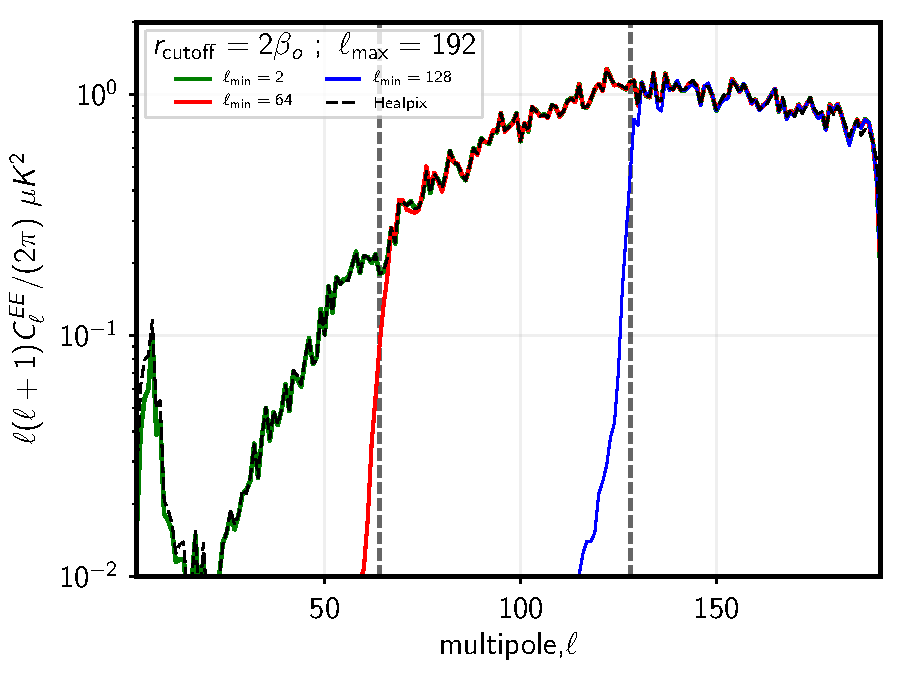
\includegraphics[width=0.49\columnwidth]{simulated/multipole_filter/eqmask/ee-spectrum-rteb-2beta_multipole_filtering.pdf}}
\subfigure[]{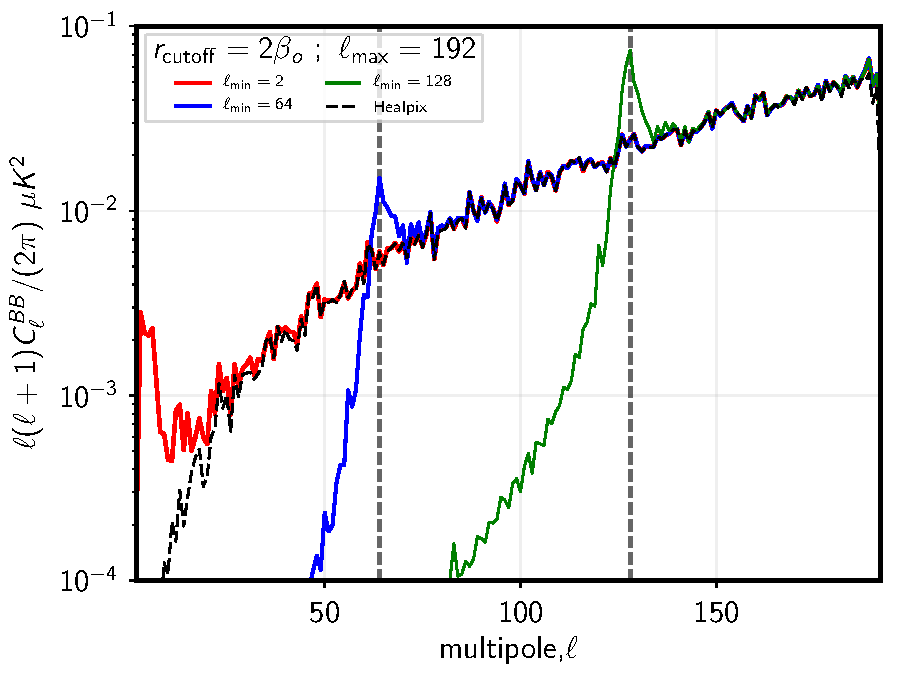
\includegraphics[width=0.49\columnwidth]{simulated/multipole_filter/eqmask/bb-spectrum-rteb-2beta_multipole_filtering.pdf}}
\subfigure[]{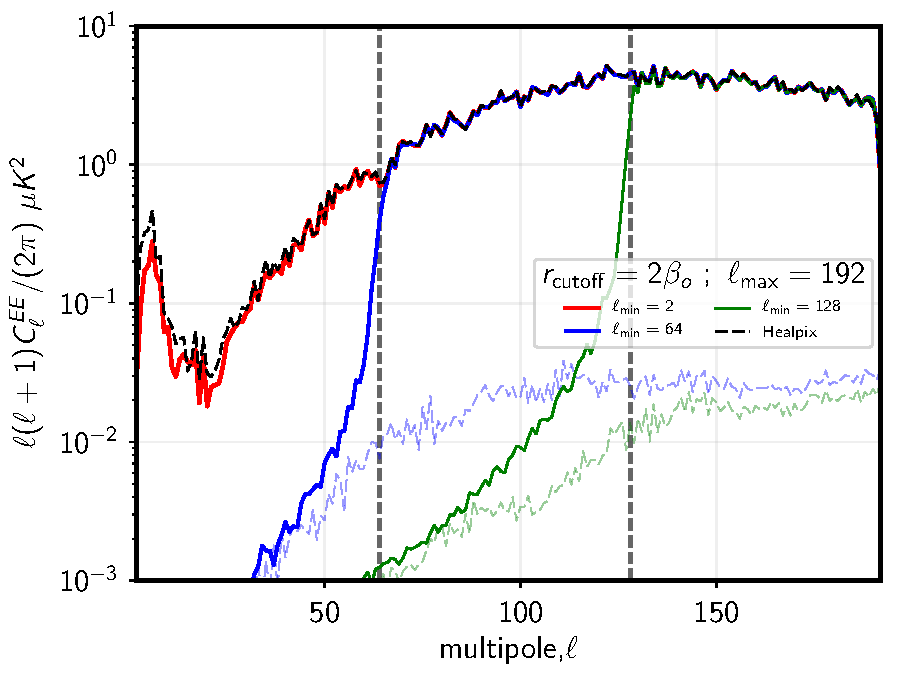
\includegraphics[width=0.49\columnwidth]{simulated/multipole_filter/eqmask/ee-spectrum-requ-2beta_multipole_filtering.pdf}}
\subfigure[]{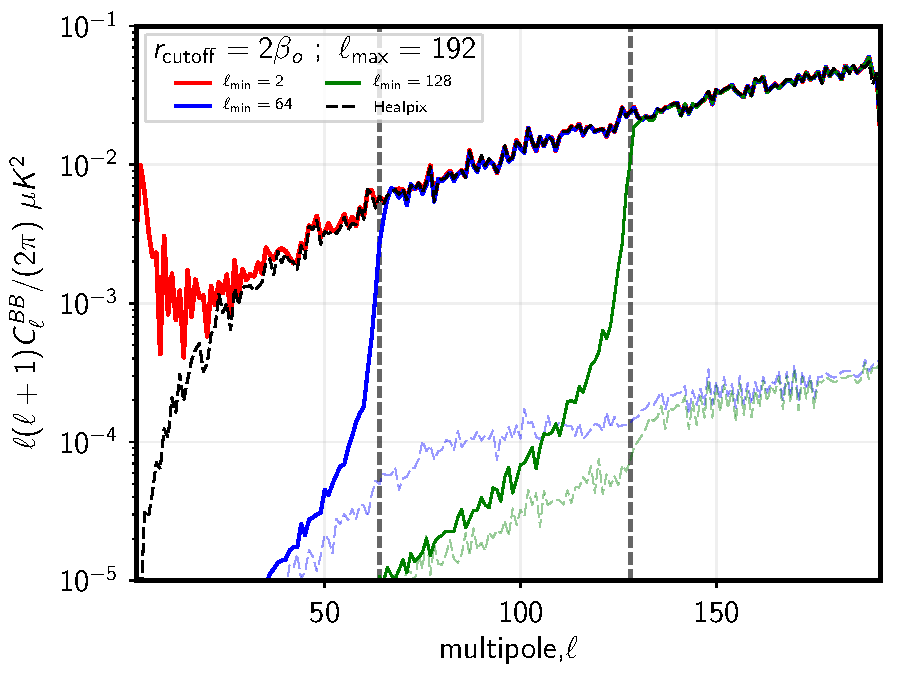
\includegraphics[width=0.49\columnwidth]{simulated/multipole_filter/eqmask/bb-spectrum-rbqu-2beta_multipole_filtering.pdf}}
\caption{The top left and right panels depict the spectra  for E and B modes respectively, where each panel shows the spectra derived from filtered E \& B maps computed using local convolutions. The bottom left and right panels depict the same for spectra derived from $[Q,U]_E$ and $[Q,U]_B$ maps computed using local convolutions. The thin dashed lines in the bottom panels depict the residual power in the orthogonal modes. The vertical gray lines mark the low multipole cut off corresponding to $\ell_{min}=64$ and $\ell_{min}=128$. All local convolution have been performed with $r_{\rm cutoff} =2 \beta_o$.}
\label{fig:filtered_spectra}
\end{figure}
%
We construct radial filters with three different low multipole cut-offs: $\ell_{\rm min} =2,64 ~ \& ~ 128$ which are depicted in \fig{fig:rad_ker_multipole_filter}. The kernels have been purposefully multiplied by a factor of the angular distance $\beta$ to highlight the differences in the radial kernels for different multipole cut-offs.

We use these different radial kernels to perform local convolutions on the simulated polarization maps. We use the same radial cut off: $r_{\rm cutoff}=2\beta_o$ for all the different filters, where $\beta_o=22.5^{\circ}$. The spectra from the filtered maps so constructed are depicted in \fig{fig:filtered_spectra}. Through these results we demonstrate how we can alter the radial part of the convolution kernels to get maps with the desired multipole filtering. \comment{What do you have to say about the jump in power for the B mode spectra at the low multipole cutoff, derived from filtered B maps ?}

%--------------------------------------------------------
%--------------------------------------------------------
